\documentclass[12pt]{article}
\usepackage[a4paper, margin=1in]{geometry}
\usepackage{graphicx}
\usepackage{enumitem}
\usepackage{hyperref}
\usepackage{titlesec}
\usepackage{fancyhdr}
\usepackage{longtable}
\usepackage{tabularx}
\usepackage{booktabs}
\usepackage{parskip}
\usepackage{color}
\usepackage{lscape}
\setlength{\headheight}{14.5pt} % <-- fixes fancyhdr warning

\pagestyle{fancy}
\fancyhead[L]{TrackIN Project Report}
\fancyhead[R]{SS 2025}
\fancyfoot[C]{\thepage}

\title{TrackIN: Development of a Tracking App and Analysis of Altitude Data}
\author{Technische Hochschule Ingolstadt \\ \textbf{Project Coordinator:} Prof. Dr. Robert Gold}
\date{Summer Semester 2025}
\begin{document}

\maketitle
\tableofcontents
\newpage

\section{Project Overview}
This project aims to develop a cross-platform tracking application. The app records satellite-based GPS data, with special focus on the algorithm and accuracy of tracking. The application is designed to run on Android initially. The team later decided to include support for iOS devices as well. Full development has been done initially in Flutter, and Java version has developed later on as simplicity. 

\subsection*{Features}
\begin{itemize}
    \item Record GPS + Altitude data
    \item View and analyze GPX files
    \item Notification system
    \item Modular UI
    \item Altitude correction using smoothing algorithm
    \item Share GPX files
\end{itemize}

\section{Installation}
To install and run the TrackIN app, follow these steps:

\subsection*{Requirements}
\begin{itemize}
    \item Flutter SDK (version X.X.X or higher)
    \item Android Studio or Xcode (for Android/iOS development)
    \item Git
\end{itemize}
\subsection*{Steps}
\begin{enumerate}
    \item Clone the repository:
    \begin{verbatim}
    git clone https://github.com/CAIProj/Frontend.git
    \end{verbatim}
    \item Navigate to the project folder:
    \begin{verbatim}
    cd Frontend
    \end{verbatim}
    \item Install dependencies:
    \begin{verbatim}
    flutter pub get
    \end{verbatim}
    \item Run the app on an emulator or physical device:
    \begin{verbatim}
    flutter run
    \end{verbatim}
\end{enumerate}
\subsection*{Note}
Make sure your development environment is configured correctly (see official Flutter docs at \url{https://docs.flutter.dev}).
\section{Project Management}
\begin{itemize}
    \item Weekly meetings every Thursday at 14:55 (Room K013)
    \item Tasks assigned to each member
    \item Working hours tracked via Google Sheets
    \item Communication in Discord/Microsoft Teams
\end{itemize}

\section{Licensing}
This project uses the MIT License. All code is open source.

\section{Notable Events}
\begin{itemize}
    \item \textbf{03.04.2025} – First GPX data recorded around campus
    \item \textbf{05.06.2025} – Project Excursion
    \begin{figure}[h!]
    \centering
    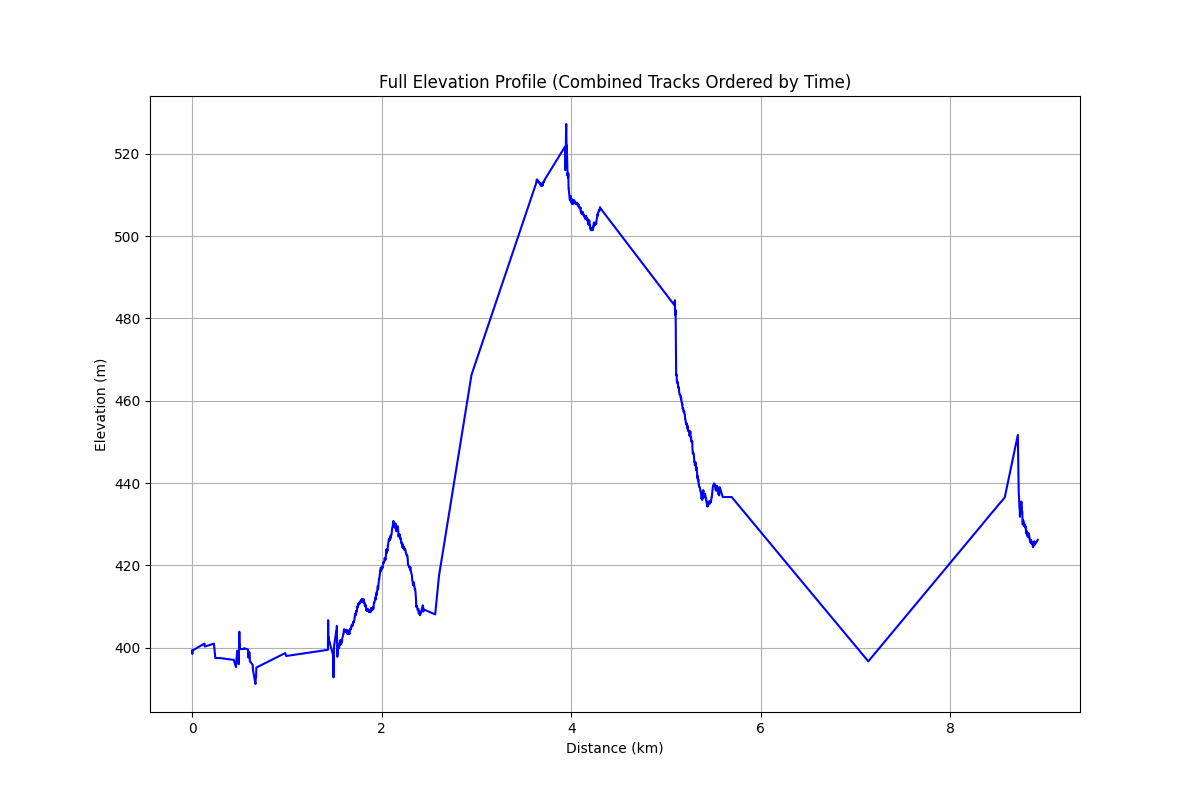
\includegraphics[width=0.8\textwidth]{Project_Screenshots/guessitworked.png}
    \caption{First GPX file recorded by our app}
\end{figure}
\end{itemize}

\newpage
\section{Project Members}
\begin{itemize}
    \item Robin Roßnagel
    \item Thomas Williams
    \item Himanka Ashan
    \item Susheel Kumar
    \item Prashil Rupapara
    \item Isaac Ye
    \item Pamirbek Almazbekov
    \item Baatarbileg Erkhembayar
    \item Syed Aayan Ahmed
\end{itemize}

\newpage
\section{Tasks and Responsibilities (Summary Table Format)}

\begin{longtable}{p{3cm} p{1.5cm} p{4cm} p{7cm}}
\toprule
\textbf{Member} & \textbf{Task ID} & \textbf{Title} & \textbf{Description \& Result} \\
\midrule
\endfirsthead
\toprule
\textbf{Member} & \textbf{Task ID} & \textbf{Title} & \textbf{Description \& Result} \\
\midrule
\endhead
Robin Roßnagel & T4 & Communication \& Tracking & Discord used for team communication; Excel for working hours. \\
& T14 & Android Dev Research & Android setup faced team device constraints; iOS prioritized. \\
& T15 & GPS \& Altimeter App & Flutter app developed; iOS tested; Android pending. \\
\midrule
Syed Aayan Ahmed & T4 & Communication \& Tracking & Same as Robin. \\
& T14 & Android Dev Research & Same as Robin. \\
& T15 & GPS \& Altimeter App & Same as Robin. \\
\midrule
Thomas Williams & T1 & Open Source License & Researched options; MIT License selected. \\
& T4 & Communication \& Tracking & Set up Discord and Excel. \\
& T6 & Altitude DB Comparison & Chose Open-Elevation; Python script written. \\
& T18a & Route Comparison & Investigated synchronizing GPX recordings. \\
& T24 & Modularization & Refactored and split Python scripts into modules. \\
\midrule
Baatarbileg Erkhembayar & T2 & Git Options & Chose GitHub after university option failed. \\
& T4 & Time Sheet Improvements & Auto-sum working hours in Excel. \\
& T5 & Altitude Reference Systems & Analyzed GPS and altimeter methods (Jupyter notebook). \\
& T12 & Git Setup & Created GitHub repos for backend, frontend, docs. \\
& T17/T18 & Curve Smoothing & Loess-v2 selected as best method (Jupyter notebook). \\
& T28 & Frontend Testing & iOS tested using Xcode and MacBook. \\
& T28+ & iOS testing & Code coverage testing\\
& T30 & Documentation & Structured this documentation. \\
& T30+ & GitHub structure & Improved the structure. \\
\midrule
Himanka Ashan & T2 & Git Options & Chose GitHub after university option failed. \\
& T4 & Time Sheet Improvements & Auto-sum working hours in Excel. \\
& T5 & Altitude Reference Systems & Analyzed GPS and altimeter methods (Jupyter notebook). \\
& T12 & Git Setup & Created GitHub repos for backend, frontend, docs. \\
& T17/T18 & Curve Smoothing & Loess v1 , Loess v2, Spline fit. \\
& Task & Curve Smoothing Evaluation & Loess-v2 selected as best method \\
& T26 & Backend Framework & Backend server implemented with FastAPI \\
& Task & Android studio java & Implemented a tracking application in android studio from scratch. \\
\midrule
Susheel Kumar & T3 & Git Structure & Suggested initial repo structure. \\
& T6 & Altitude DBs & Researched databases: SRTM, ASTER, Copernicus, etc. \\
& T16 & Use Case Diagram for Tracking App & App’s operational workflow. \\
& T23 & Modules of app & Modularization of app. \\
& T23 & Class diagram for Tracking App &  Created class diagram for the tracking app. \\
& T27 & Backend Testing & Test plan created  \\
& Task & Backend Testing & 3 tests (plotter.py, models.py, evelation\_api.py) documented  \\
\midrule
Prashil Rupapara & T3 & Git Structure & Suggested initial repo structure. \\
& T6 & Altitude DBs & Researched databases: SRTM, ASTER, Copernicus, etc. \\
& T16 & Use Case Diagram for Tracking App & App’s operational workflow. \\
& T23 & Modules of app & Modularization of app. \\
& T23 & Class diagram for Tracking App &  Created class diagram for the tracking app. \\
& T24 & Unifying scripts & Unified the scripts of the backend and update it if needed. \\
& Task & Pull request merging & Merged pull requests for backend repo. \\
& Task & Final Unification & Did final unification needed after addition of synchronised plotting. \\
& Task & Update plotting with main & Added functionality to have multipe plots(with any of the api and smoothing method) with CLI usage. \\
& Task & Python dependency management & Made possible to have easy ython setup locally with just few commands in terminal. \\
& Task & Create class diagram & Created class diagram with the relationship in between for backend. \\
& Task & Update README.md & Updated and added needed information and links in README.md file. \\
\midrule
Isaac Ye & T8 & GPX file parsing logic & Wrote parsing logic, distance vs elevation graph. \\
& T22 & UI prototypes for use cases & Created prototypes according to T16. \\
& T25 & App Review\& Fixes & Testing, reviewing, giving feedback to the app \\
& Task & Andriod fixes & Changed a dependency not supported on Android.\\
& Task & Flutter app & Modularized codebase and added more pages \\ 
& Task & Flutter app & Added notification system, initial UI changes and fixes. \\
& Task & Flutter app & Business logic fixes and remove deprecated status state. Mostly finalized UI change and fixes.\\
& Task & Flutter app & Changes to interact with the Framework backend.\\         
& Task & Flutter app & Improved local-upload GPX file mapping and optimized UI.\\   
\midrule
Pamirbek Almazbekov & T8 & GPX file parsing logic & Wrote parsing logic, distance vs elevation graph. \\
& T22 & UI prototypes for use cases & Linking to UML diagram from T16. \\
& T25 & App Review\& Fixes & Testing, reviewing, giving feedback to the app \\
& T29 & Technical Docs & Wrote technical documentation. \\
& Task & Android studio java & Implemented a tracking application in android studio from scratch. \\

\bottomrule
\end{longtable}

\subsection*{Detailed task summary}
{\large\textbf{Isaac Ye}}
T8: Wrote a Python helper file that included GPX file parsing and graph plotting.

T22: Following the UML diagram in T16, we created UI prototypes for the Flutter application using Figma for multiple pages, such as the home page (idle state), home page (recording state), a page displaying all local GPX files, and a page for displaying detailed information for a selected GPX file. These prototypes are summarized with their respective use cases in a use case document. Some changes were made to UML diagram as well to include missing use cases.

T25: Tested and reviewed the Flutter application on Android (emulated) and Chrome and provided feedback.

Android Fixes: Changed a dependency that was not supported on Android, which made the Flutter application work on the Android platform.

Flutter App: Reorganized the codebase from a singular main file to be more modular, added two new pages (one for displaying all recorded tracks, one that displayed information about individual tracks), and started to change the UI to be closer to the UI prototypes.

Flutter App: Add new notification system for displaying messages, ‘Are you sure?’ dialogue when deleting a track, fixed filepicker dependency on Android when importing a GPX file, and implement initial home UI changes.

Flutter App: Fixes to stopwatch logic, moved legacy status messages to notifications instead, and disallow recording UI to be shown if location permission is denied.

Flutter App: Fixed display of statistics and convert timestamps of GPX files from UTC to local time, worked to finalizing the styling of the home page, tracks page and track page.

Flutter App: Removed point limit for a recording and allowed tracking while not in the application (only on Android, this feature for iOS would require a Apple Dev account, which requires a fee of €100 per year). Changed GPS to stream instead of querying for the location and changed the GPS query interval to be less frequent. Limited the amount of points rendered for the widget displaying detailed point information (since we could have infinite points).

Flutter App: Added a client for interacting with the Framework to upload GPX files. Added an account page (to login and register to interact with the Framework). Added buttons to upload / delete files to / from the Framework, which only allows the user to do so if logged in. Attempted to map local files to uploaded files (to ensure we don't upload twice and can delete them). The approach used would fail in the case where the user switches accounts, however. More UI fixes and cleaning up.

Flutter App: Instead of managing a local file that holds the mapping of local to uploaded files, I opted to download the remote files on login and use hashing to compare the contents of GPX files (which fixes the case of switching accounts). Loading the tracks page now doesn't try to spawn too many threads that it hangs the render thread. Added header text to statistics for clarity.

{\large\textbf{Himanka Ashan}}
Research Git options. 
Result: GitHub used due to lack of university contact 

Research altitude reference systems and techniques 
Result: Comprehensive explanation of altitude tracking systems, including the reasoning on the difference between actual elevation and elevation from apis 

Set up Git 
Results: Created and managed repositories in github 

Curve smoothing algorithms 
Results: implemented custom smoothing algorithms. Namely, Loess v1 , Loess v2, Spline fit.  All algorithms are implemented in a way that they can be imported easily. 

Evaluate smoothing algorithms 
Results: Applied mean error and mean squared error to evaluate the smoothing algorithms. Loess v2 was proven to be better from the evaluation report. 

Framework 
Results: Backend server implemented with FastAPI with following methods 

- POST /register : Register a user 

- POST /login : Login method  POST /upload : Upload a gpx file to the database 

- GET /files/ : Return all files from a user 

- GET /files/fileid : Return Specific GPX file and download 

- DELETE /files/fileid : Deletes a gpx file from database 
Hosting the server : Used Render.com’s free hosting account to deploy the server on the internet. Special render configuration was needed. 

Android Studio Java Application (2-weeks) 
Results: Implemented a tracking application in android studio from scratch. 
- Introduced Altitude measurement to the app and adapted the database and the receiver 

- Dynamic START/STOP button to start tracking 

- App Structuring: Introduced Fragments (TrackFragment, DashboardFragment) 

- Added Accumulating time and distance to the tracking page (Haversine distance) 

- Altitude, Lat:long, Distance, Time are displayed in stylish cards to present a modern look 

- UI improvements 

- Code cleanups

{\large\textbf{Susheel Kumar, Prashil Rupapara}}
Git research
We decided on how our project on Git should be structured and what should be the rules of using git, the result was rules and directory structure of git project

Freely accessible databases
We identified freely accessible altitude databases and evaluate their accuracy. The findings revealed variations in altitude precision among available resources, with some datasets offering higher resolution for specific regions. Open-source accessibility played a key role in determining the usability of the databases, providing valuable data for geographic and environmental analysis. The comparison underscores the importance of selecting appropriate altitude datasets based on accuracy requirements and intended applications.

Use case diagram
We created a detailed use case diagram was developed for the Android tracking app, outlining complete use cases and their corresponding actions. The diagram specifies interactions between users, system components, and key functionalities, providing a structured representation of the app’s operational workflow.

Modules of app
We had to determine different modules of the app so that they could be assigned to different development teams, the result was modularization of app and suggestion for tasks which could be assigned to different teams

{\large\textbf{Susheel Kumar}}
Backend test plan
A test plan was developed to evaluate the backend functionality of the app. Key features requiring testing were identified, and appropriate test approaches were determined to ensure comprehensive validation. The plan aimed to enhance reliability, optimize system performance, and address potential issues before deployment.

{\large\textbf{Prashil Rupapara}}
Extensive contributions were made to the backend structure, CLI plotting functionality, environment setup, and project documentation, with a focus on maintainability, usability, and modular design.

Various backend Python scripts—including those for GPX parsing, elevation API integration, smoothing, and plotting—were unified into a modular and logically structured architecture. Final refactoring was performed after the addition of synchronized plotting capabilities to maintain a coherent and testable codebase.

The command-line interface (\texttt{main.py}) was extended to support multiple elevation sources and smoothing techniques such as \texttt{--add-openelevation} and \texttt{--add-loess1}. For synchronized plotting, validation logic was implemented to ensure only one comparison source could be used at a time, while non-synced plotting supports multiple sources simultaneously. These enhancements provided a flexible and user-friendly CLI experience.

Python dependency management was handled using \texttt{Poetry}. Both \texttt{pyproject.toml} and \texttt{requirements.txt} files were added to support different setup preferences. The environment setup was tested and verified on Windows 11 machine.

UML class diagrams for backend components were created independently using Mermaid syntax. Key classes such as \texttt{Track}, \texttt{ElevationProfile}, \texttt{OpenStreetMapElevationAPI}, and \texttt{Plotter}  were included, along with their internal relationships. These diagrams served as a useful reference for both implementation and documentation.

The \texttt{README.md} file was updated to include local development setup instructions, links to example Jupyter notebooks, and embedded references to backend class diagram files. These documentation efforts enhanced onboarding and usability for future contributors.

{\large\textbf{Tom Williams}}
Deciding which License to use.
Under the directive that the license must be open source, I looked into the different kinds of open source license available to use. I wrote a summary of the different kinds, which generally came under the categories of "Permissive" and "Copyleft", and their advantages and disadvantages. I presented my findings to the team, giving my thoughts on which license we should use, and we all agreed to use the MIT License.

Research freely accessible altitude databases
I looked into which altitude databases we could use to compare our recorded data with to measure the accuracy. I found Open-Elevation, OpenTopography, NASA Earth data, and Google Earth engine. I found that Open-Elevation was the best to use as the API was easy to use and it returned numerical data from the request that we could use. Whereas OpenTopography for example, would only return an image representing topographical data which would have required a lot more work to implement and risked not working at all. The other APIs either didn't offer the geographical region I was working with, or provided identical data to Open-Elevation, so I decided we should only use Open-Elevation and I wrote a script that would plot the elevations from the GPX recording alongside the elevations provided by the API.

Modularisation of the python scripts
As I had done the GPX file processing, plotting, API calls and command line parsing all in a single file, I worked to separate the functionality into separate files to keep the code clean and easy to read.

Improving plot functionality
As part of my plotting programme, I tried to find a way to plot two different gpx files of the same, or a similar route, in a way that made sense. I tried to implement a strategy of having a primary plot and a secondary plot, where the secondary plot would only show on the graph when it was within a certain distance of the primary plot, and leave gaps where the two plots diverged, so the elevations would represent the same geographical spot. But this turned out to be incredibly difficult, and after discussing with the team, we decided that we would leave this idea for now, try to implement a simpler way of plotting two routes for comparison, and if time permits, try to solve this strategy later.

{\large\textbf{Baatarbileg Erkhembayar}}

Git Options
We considered using the University's GitLab instance, but due to unsuccessful contact with Prof.\ Dr.\ Sebastian Apel, we opted for GitHub.

Working Hours Excel:
A simple summary table was created for automatic calculation of working hours.

Reference Systems
Several reference systems were identified, introduced, and evaluated using a Jupyter notebook.

GitHub
https://github.com/CAIProj – Three repositories were created: \textit{Backend}, \textit{Frontend}, and \textit{Docs}. All findings and documentation are stored in the \textit{Docs} repository.

Curve Smoothing: \texttt{curve\_smoothing\_algo.ipynb} was developed to compare different curve smoothing algorithms. The \textit{Loess-v2} algorithm performed best.

Frontend Testing Plan
The task was similar to T25. Simulator testing was successful; however, testing on a real iOS device was not possible due to incomplete app state requiring debugging.
After the modification with the real phone connection, using Apple developer tools, I downloaded the app locally and tested with test cases. More appear in Testing section

Project Documentation
This document serves as the official project documentation. Project is written in Latex, and uploaded into Github with supporting photos as a zip file.

Frontend iOS Testing
iOS frontend was tested using a MacBook and Xcode. Test cases were created, and code coverage analysis was performed. Code coverage only had 12 percent, which is due to having less test cases in widget.test app. 

\vspace{1em}

{\large\textbf{Syed  Aayan Ahmed, Robin Roßnagel }}
During the implementation of our cross-platform tracking application, we developed a modular and extensible system for recording, processing, and comparing geospatial data,
specifically targeting GNSS-derived altitude values. The app was built using Flutter to ensure native performance on both Android and iOS, with backend logic primarily written in Dart
and integration of native plugins where required.

We implemented a persistent background tracking service using Dart Isolates incombination with the flutterforegroundtask package. This design allowed the app to collect GPS coordinates and altitude data (from GNSS) at 5-second intervals, even when running in the background or with the screen off. The service communicated with the main
isolate using a ReceivePort, ensuring asynchronous, thread-safe data flow. Each recorded point was time-stamped and included latitude, longitude, and altitude. The location stream
was sourced via the geolocator package, with accuracy settings tuned to LocationAccuracy.best for maximum vertical resolution

1. Track Alignment Function:
We implemented aligntrackendpoints, which processes two GPX tracks and
truncates them such that both start and end at approximately the same spatial
positions. The algorithm performs a bi-directional search within the first and last 20%
of each track to identify the closest start and end pairs within a configurable
threshold (default: 100 meters). These indices are then used to slice the point arrays,
resulting in aligned sub-tracks suitable for direct comparison. Robust error handling
was added to manage edge cases such as non-overlapping routes, insufficient point
density, or excessive drift.

2. Track Interpolation Function:
We further implemented interpolatetomatchpoints, an algorithm that resamples
the second track to ensure it has the same number of points as the first. This is
accomplished using cumulative arc-length interpolation based on Haversine distance.
The resampled track maintains spatial continuity and allows for pointwise analysis
(e.g., elevation delta at fixed intervals), which is crucial for evaluating vertical
accuracy and identifying anomalies.

In parallel, we addressed several practical implementation challenges. The Android-specific
foreground service required careful lifecycle management to ensure it remained active
under aggressive power management policies. We also resolved early-stage issues related to
file handling and serialization of GPX data, particularly on Android 13+, where scoped
storage restrictions affected write permissions. We migrated file writing to use
pathprovider and ensured compliance with platform-specific permissions. The GPS 

sampling interval and filter thresholds were empirically tuned to balance temporal
resolution, power consumption, and altitude stability.
To verify the correctness and reliability of our implementation, we developed a
comprehensive test suite comprising over eight unit and integration tests. These covered a
range of scenarios: identical tracks, varying sampling densities, partial overlaps, route drift,
noise-injected altitude profiles, and real-world walking/cycling recordings. All tests were
successfully validated, and debug visualizations were used to qualitatively assess alignment
and interpolation performance.
The resulting application and backend form a complete open-source framework for altitudefocused GPS analysis and provide a solid foundation for the integration of rule-based or AIassisted correction techniques in future work.

\newpage
\section{Use case diagram}
\begin{figure}[h!]
    \centering
    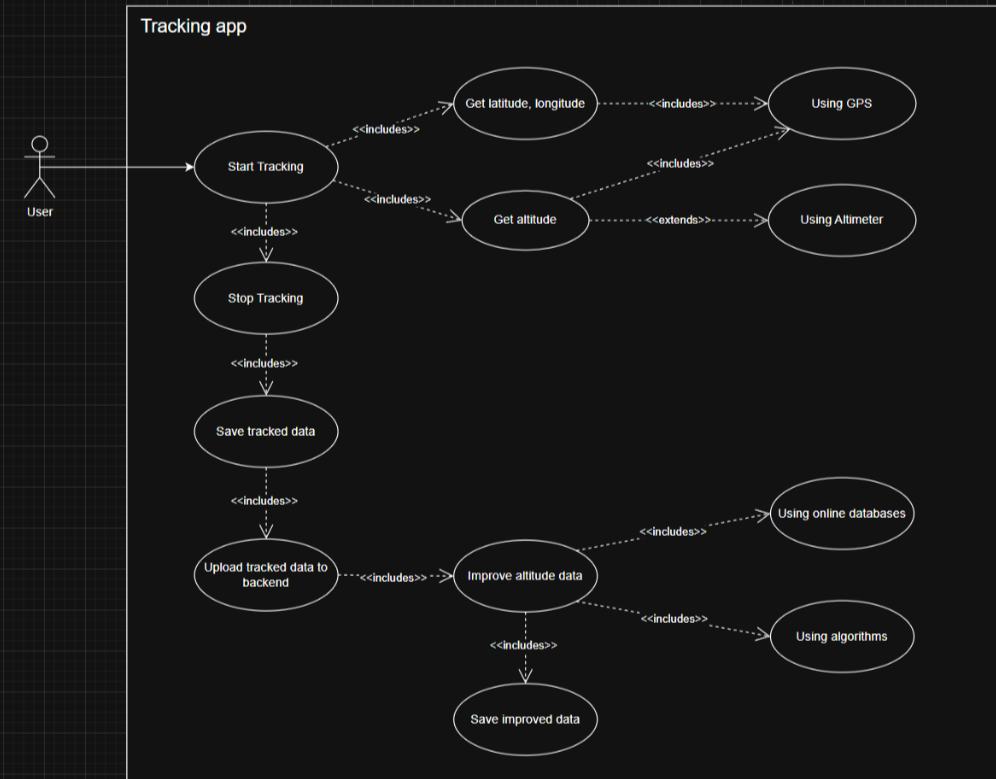
\includegraphics[width=\textwidth]{Project_Screenshots/usecase.png}
    \caption{Use case diagram for TrackIN}
\end{figure}

\begin{table}[h!]
\centering
\begin{tabular}{|p{3cm}|p{11cm}|}
\hline
\textbf{Field} & \textbf{Description} \\
\hline
\textbf{Use Case}   & Home Screen Behavior Based on Time of Day \\
\hline
\textbf{Description} & The system displays one of the screens shown upon start-up (home screen), depending on the time of day. \\
\hline
\textbf{Precondition} & The user starts the application. \\
\hline
\textbf{Sequence} & N/A \\
\hline
\textbf{Postcondition} & The user has the choice to start a recording (tap and hold) or view any previous recordings (swipe left). \\
\hline
\textbf{Comments} & Colours here aren’t final and just suggestions for morning / afternoon / evening. It’s also possible to just have a grayscaled theme (see below use cases). The “swipe left to see recordings” could be replaced by having an icon in the top right corner. \\
\hline
\end{tabular}
\caption{Use Case: Home Screen Behavior}
\end{table}

\begin{figure}[h!]
    \centering
    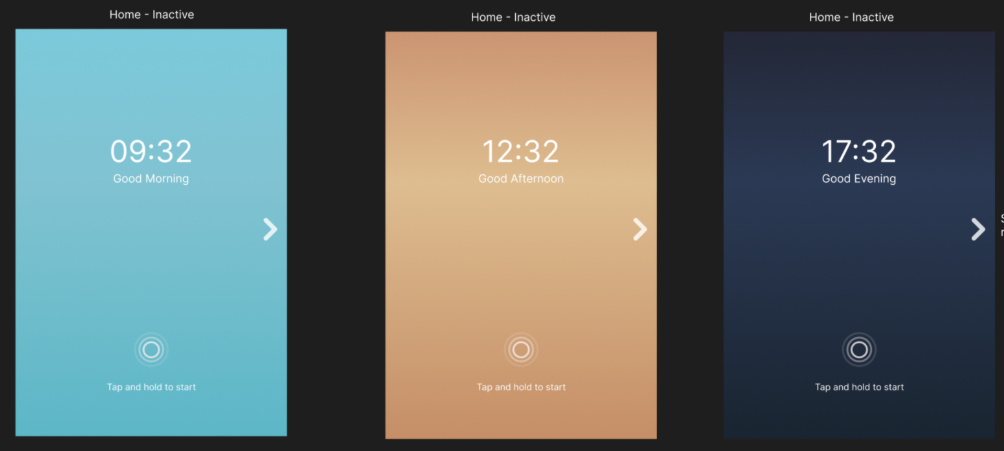
\includegraphics[width=\textwidth]{Project_Screenshots/GUIconcept.png}
    \caption{Home screen concepts}
\end{figure}

\begin{table}[h!]
\centering
\begin{tabular}{|p{3cm}|p{11cm}|}
\hline
\textbf{Field} & \textbf{Description} \\
\hline
\textbf{Use Case}   & Track Recording \\
\hline
\textbf{Description} & The application records a track. \\
\hline
\textbf{Precondition} & The application is in the idle state (on the home screen) and is not in the recording state. \\
\hline
\textbf{Sequence} & While in the idle state, the user taps and holds the circle shown on the screen (see previous use case). The application starts recording the current position and elevation through GPS (and altimeter if applicable), displays the current time, distance and elevation through text and a graph. \\
\hline
\textbf{Postcondition} & Swiping up results in the termination of the recording, saves the recorded data and returns to the idle home screen. \\
\hline
\textbf{Comments} & The colour here is grayscaled, which can either be in the final design or replaced by the alternating colours shown in the previous use case. The top right icon displays the current GPS signal strength. \\
\hline
\end{tabular}
\caption{Use Case: Track Recording}
\end{table}

\begin{table}[h!]
\centering
\begin{tabular}{|p{3cm}|p{11cm}|}
\hline
\textbf{Field} & \textbf{Description} \\
\hline
\textbf{Use Case}   & Saving and Uploading Data \\
\hline
\textbf{Description} & The application saves the recorded track. \\
\hline
\textbf{Precondition} & The application was previously recording. \\
\hline
\textbf{Sequence} & While recording, the user swipes up to terminate the recording and saves the track. The application saves the data locally onto the device. The application uploads the data to the backend. \\
\hline
\textbf{Postcondition} & The user can view the saved data and it is visible on the backend. \\
\hline
\textbf{Comments} & N/A \\
\hline
\end{tabular}
\caption{Use Case: Saving and Uploading Data}
\end{table}

\begin{figure}[h!]
    \centering
    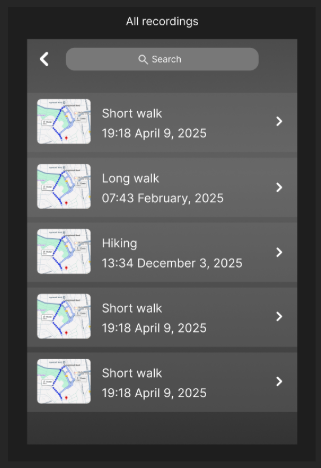
\includegraphics[width=\textwidth]{Project_Screenshots/recording.png}
    \caption{Saving, uploading data}
\end{figure}
\begin{table}[h!]
\centering
\begin{tabular}{|p{3cm}|p{11cm}|}
\hline
\textbf{Field} & \textbf{Description} \\
\hline
\textbf{Use Case}   & Viewing Recordings \\
\hline
\textbf{Description} & The application displays a list of all recordings. \\
\hline
\textbf{Precondition} & The application is in the idle state and is not actively recording a track. \\
\hline
\textbf{Sequence} & While in the idle state, the user swipes towards the left direction. \\
\hline
\textbf{Postcondition} & The user can inspect any of the listed recordings or return to the home screen (back button). \\
\hline
\textbf{Comments} & The colour here is grayscaled, which can either be in the final design or replaced by the alternating colours shown in the first use case. The button on the top left could be replaced with swiping towards the right to return to the home screen. \\
\hline
\end{tabular}
\caption{Use Case: Viewing Recordings}
\end{table}

\begin{table}[h!]
\centering
\begin{tabular}{|p{3cm}|p{11cm}|}
\hline
\textbf{Field} & \textbf{Description} \\
\hline
\textbf{Use Case}   & Viewing Track Details \\
\hline
\textbf{Description} & The application displays more details about a selected recorded track. \\
\hline
\textbf{Precondition} & There exists at least one recorded track. \\
\hline
\textbf{Sequence} & While in the list of all recordings (see previous use case), the user clicks on any of the displayed recordings. \\
\hline
\textbf{Postcondition} & The user has the option to rename, share, delete, or export the track to GPX. \\
\hline
\textbf{Comments} & The ‘share’ button and ‘export to GPX’ button could be merged. The presence of an altimeter is shown here as well (the last icon, next to ‘Has’). This icon could be changed if it isn’t clear enough. \\
\hline
\end{tabular}
\caption{Use Case: Viewing Track Details}
\end{table}

\begin{table}[h!]
\centering
\begin{tabular}{|p{3cm}|p{11cm}|}
\hline
\textbf{Field} & \textbf{Description} \\
\hline
\textbf{Use Case}   & Post-Processing Data \\
\hline
\textbf{Description} & Tracks on the backend are processed. \\
\hline
\textbf{Precondition} & The application client(s) has uploaded tracks to the backend. \\
\hline
\textbf{Sequence} & Upon track upload, the backend uses data from external databases and/or smoothing algorithms to correct the elevation according to the current position of the user. \\
\hline
\textbf{Postcondition} & The data can be analyzed further and visualized through graphs. \\
\hline
\textbf{Comments} & Figure out backend server hosting solution. \\
\hline
\end{tabular}
\caption{Use Case: Post-Processing Data}
\end{table}

\begin{figure}[h!]
    \centering
    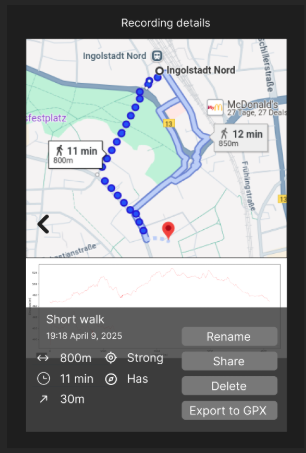
\includegraphics[width=\textwidth]{Project_Screenshots/recordingdata.png}
    \caption{Track details, Post-processing}
\end{figure}

\clearpage
\section{Backend Class Diagrams}

The following UML diagrams provide an overview of the core backend components implemented in this project. These class diagrams cover data models, elevation APIs, and plotting logic.

\begin{figure}[h!]
    \centering
    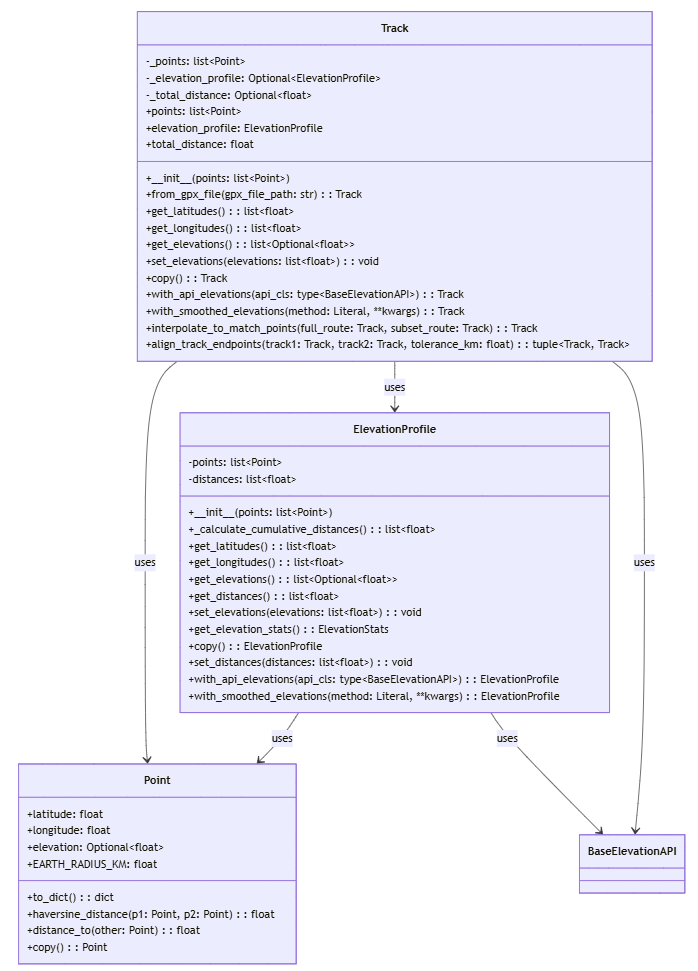
\includegraphics[height=0.8\textheight]{Project_Screenshots/class_diagram_models.png}
    \caption{Class diagram of backend data models (\texttt{Point}, \texttt{Track}, \texttt{ElevationProfile})}
\end{figure}

\begin{figure}[h!]
    \centering
    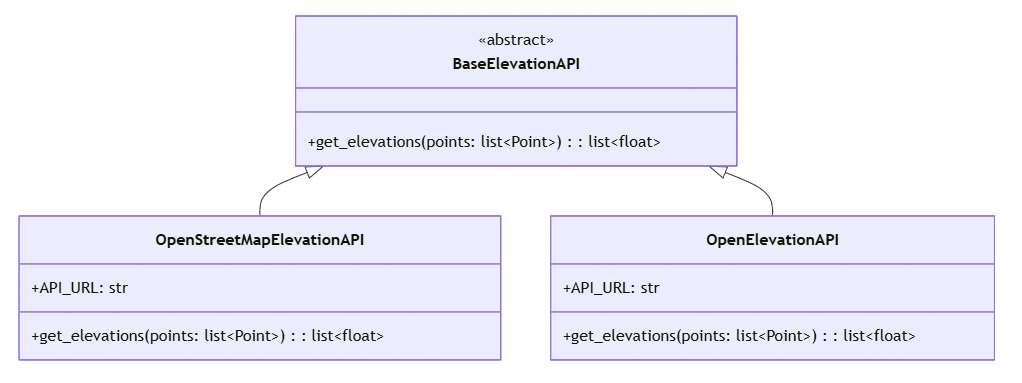
\includegraphics[width=\textwidth]{Project_Screenshots/class_diagram_elevation_apis.png}
    \caption{Class diagram of elevation API components (\texttt{OpenElevationAPI}, \texttt{OpenElevationAPI}, etc.)}
\end{figure}

\begin{figure}[h!]
    \centering
    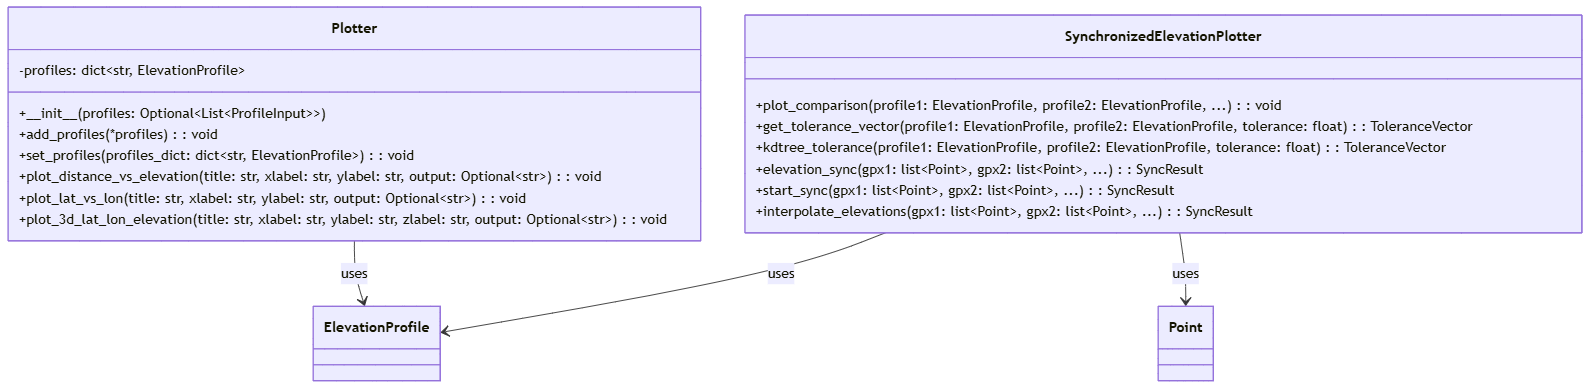
\includegraphics[width=\textwidth]{Project_Screenshots/class_diagram_plotter.png}
    \caption{Class diagram of plotting classes (\texttt{Plotter}, \texttt{SynchronizedElevationPlotter})}
\end{figure}

\clearpage
\newpage
\section{Plotting}
\begin{figure}[h!]
    \centering
    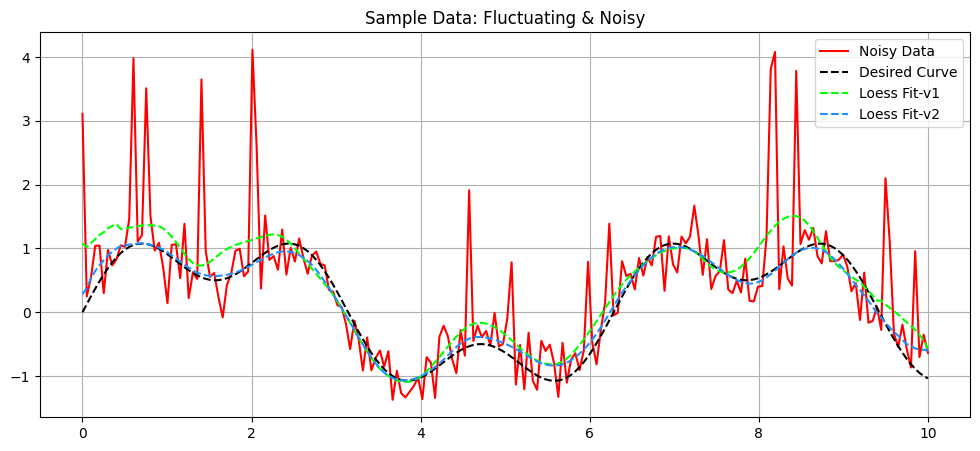
\includegraphics[width=\textwidth]{Project_Screenshots/curve_smooth.png}
    \caption{Curve smoothing algorithms}
\end{figure}
\begin{figure}[h!]
    \centering
    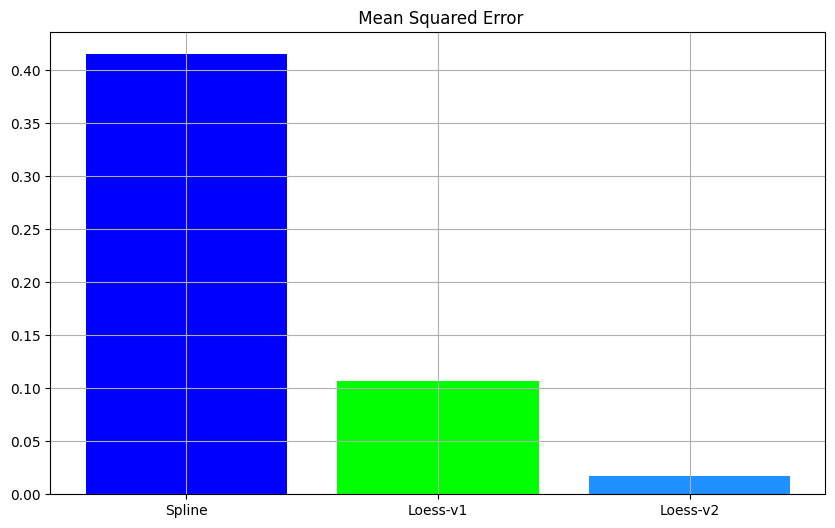
\includegraphics[width=\textwidth]{Project_Screenshots/curve smooth 2.png}
    \caption{Curve smoothing algorithm evaluations}
\end{figure}
\begin{figure}[h!]
    \centering
    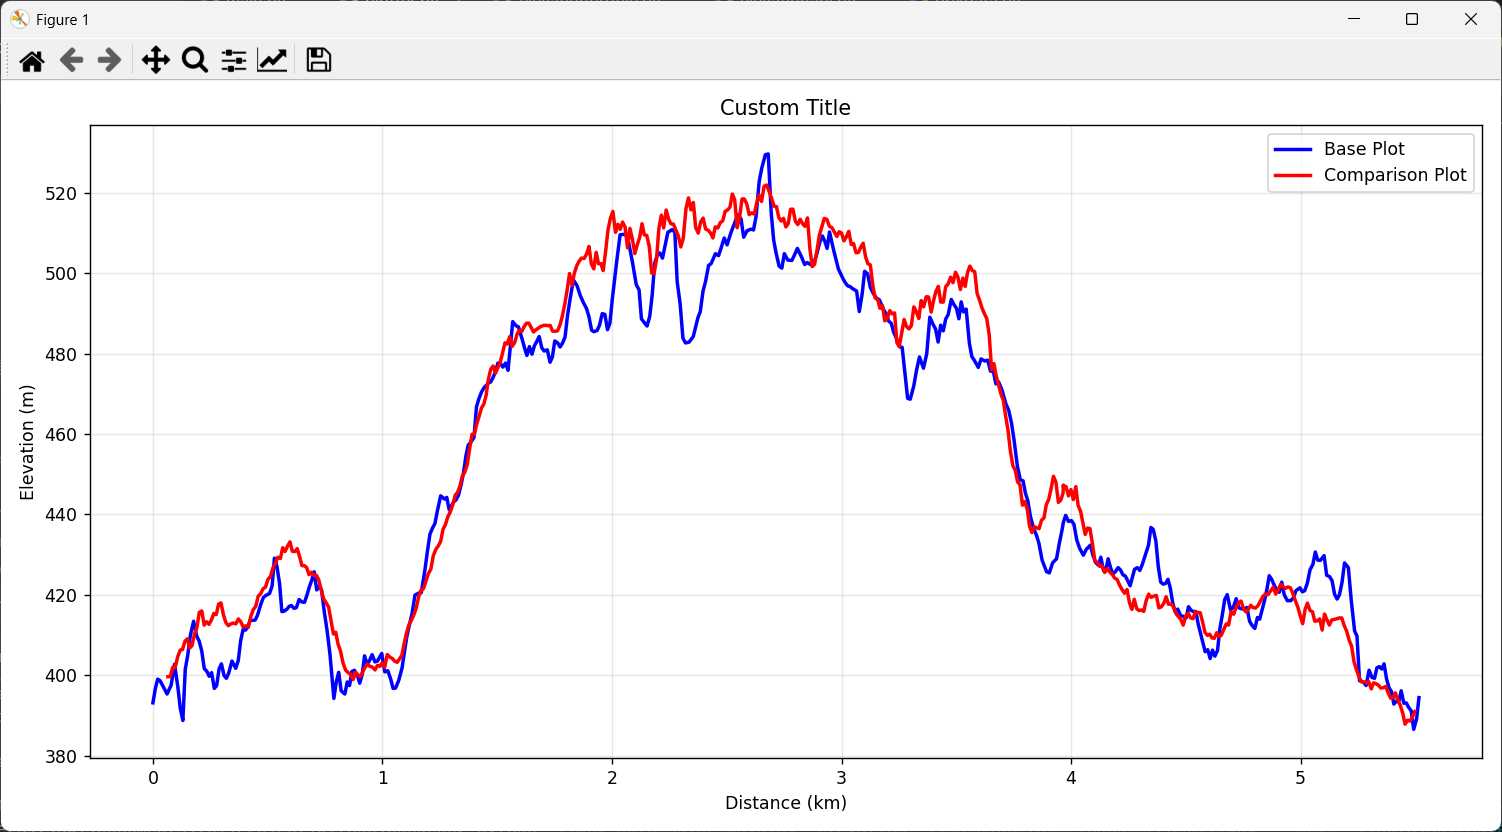
\includegraphics[width=\textwidth]{Project_Screenshots/sync.png}
    \caption{Elevation plot with Elevation sync}
\end{figure}

\begin{figure}[h!]
    \centering
    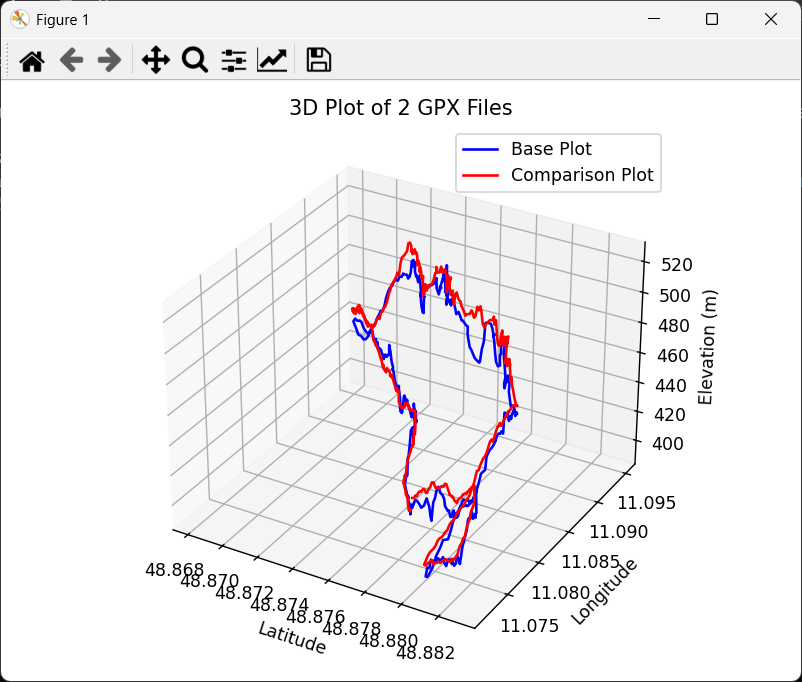
\includegraphics[width=\textwidth]{Project_Screenshots/3d plot.png}
    \caption{Comparison 3D plot	}
\end{figure}

\begin{figure}[h!]
    \centering
    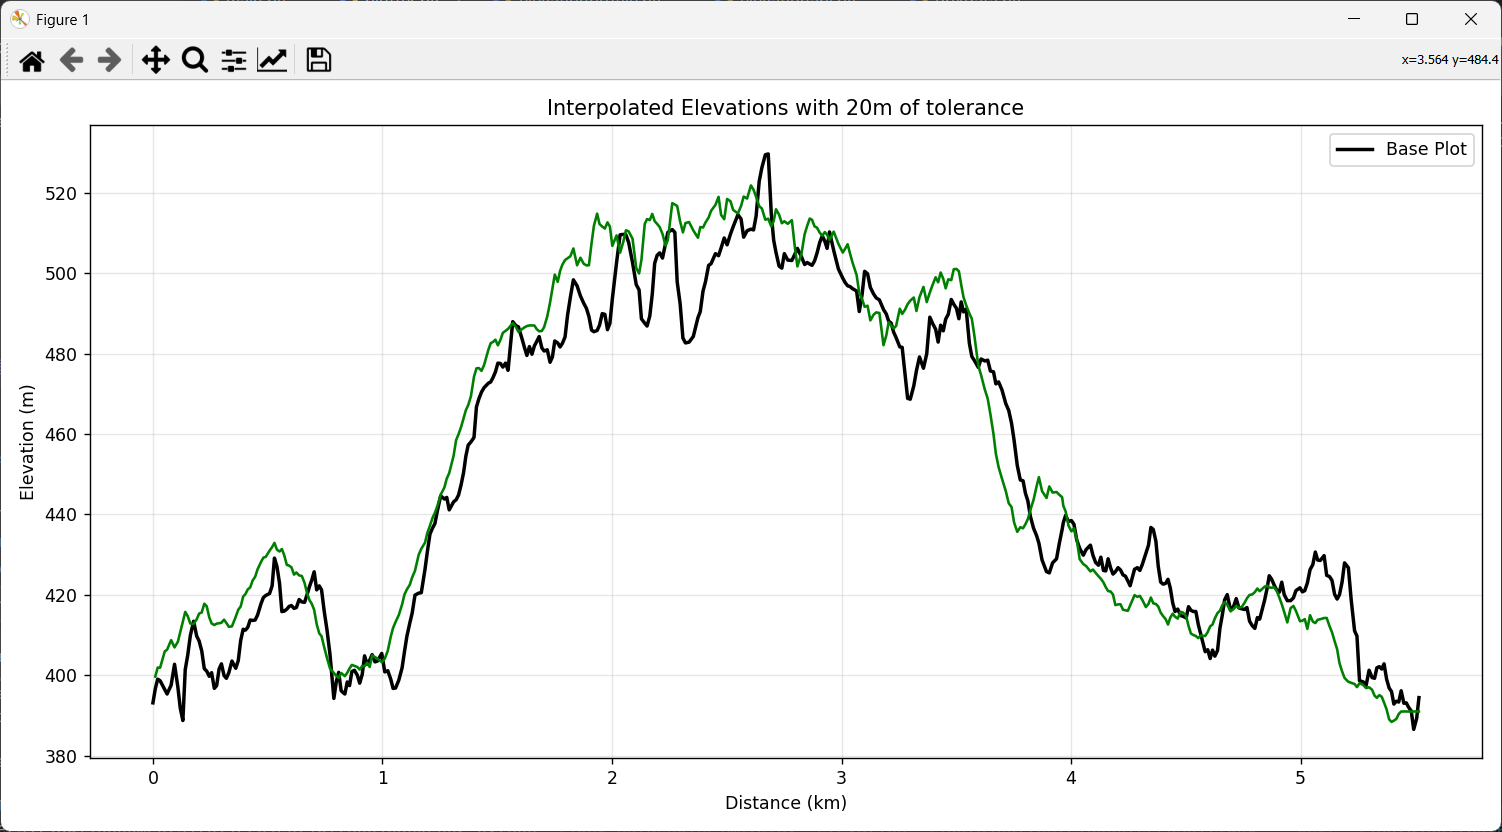
\includegraphics[width=\textwidth]{Project_Screenshots/4ElevationPlotwInterpolatedElevationsandTolerance.png}
    \caption{Elevation Plot with Interpolated Elevations and Tolerance}
\end{figure}

\begin{figure}[h!]
    \centering
    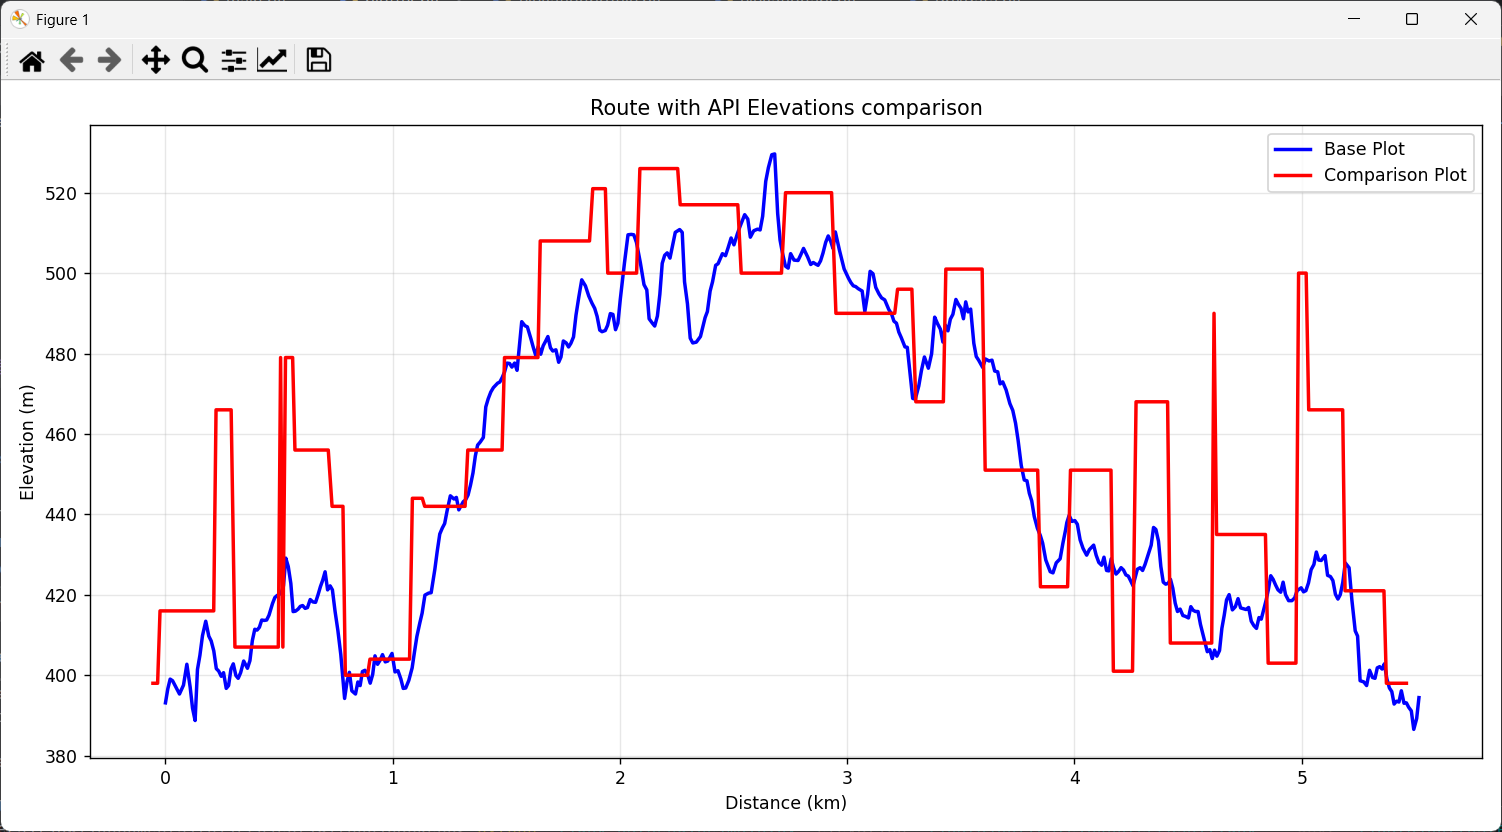
\includegraphics[width=\textwidth]{Project_Screenshots/5ElevationPLotusingAPIplot.png}
    \caption{Elevation PLotusing API plot}
\end{figure}

\begin{figure}[h!]
    \centering
    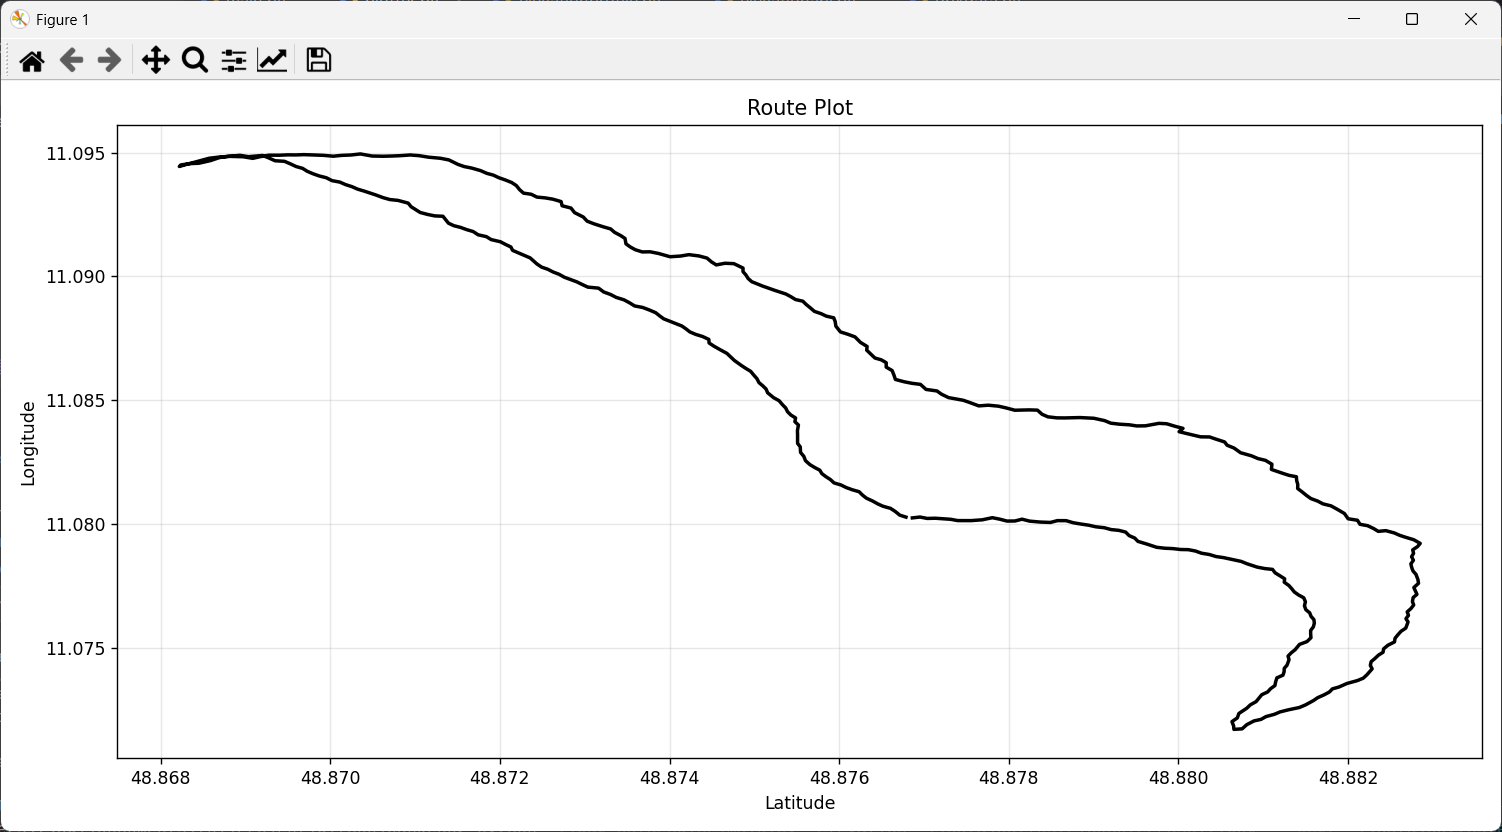
\includegraphics[width=\textwidth]{Project_Screenshots/7SingleSurfacePlot.png}
    \caption{Single surface plot}
\end{figure}

\begin{figure}[h!]
    \centering
    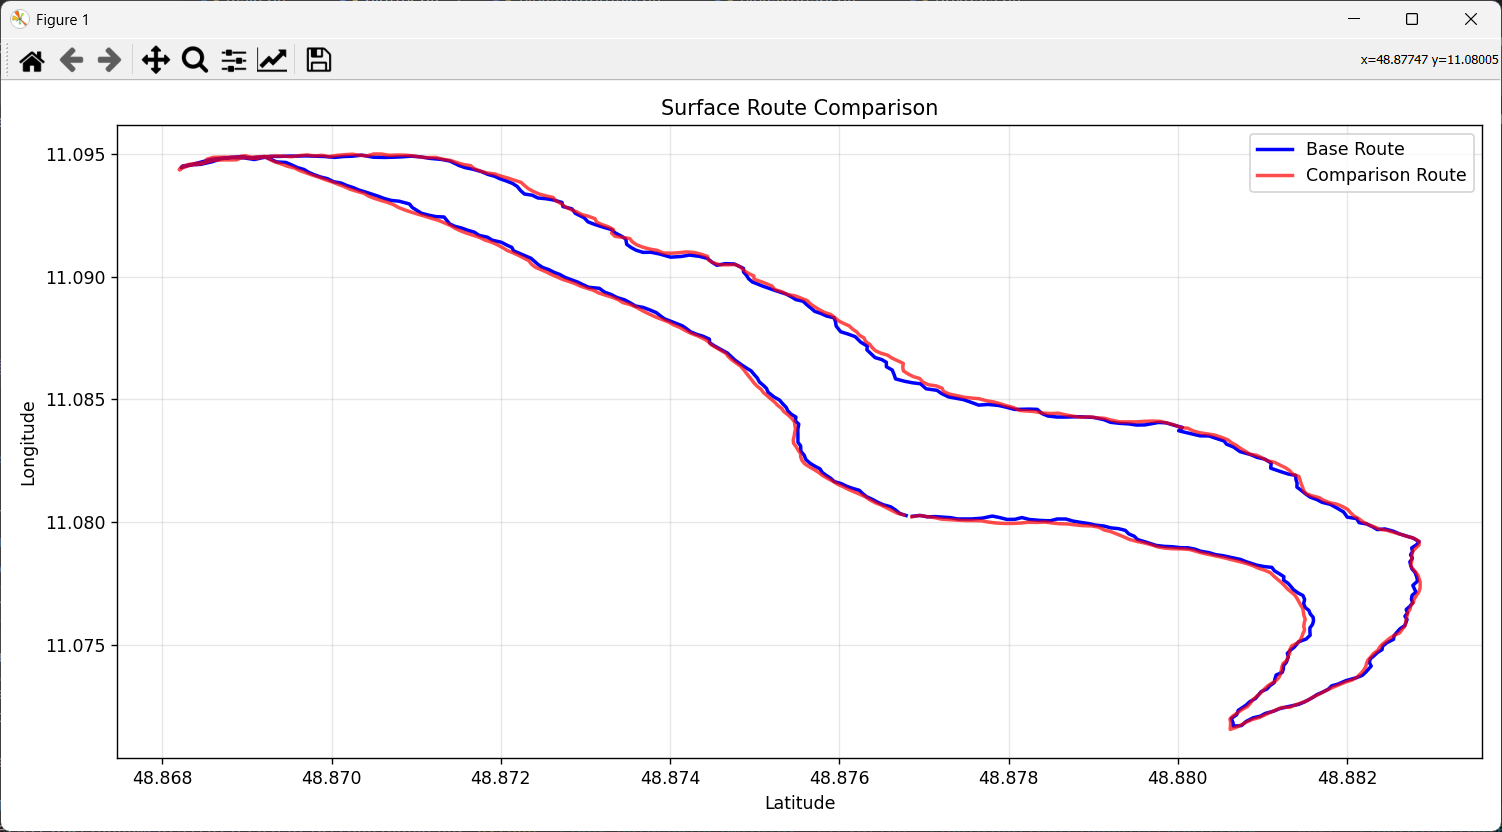
\includegraphics[width=\textwidth]{Project_Screenshots/6SurfacePlotComparisonPlot.png}
    \caption{Surface comparison plot}
\end{figure}

\clearpage

 \noindent\textbf{Tom Williams:} analysing discrepancies in recorded elevations. To ensure flexibility, I designed the system with optional divergence detection, beyond a user-defined tolerance, allowing users to focus solely on plotting the tracks if desired. The final tool offers three synchronisation methods, each with their own pros and cons, two divergence measurement options, an argument parser supporting various plot types, synchronisation methods, and tolerance settings inputted in the command line and the choice to either display graphs on screen or save them for later use. This modular approach provides users with adaptable and precise control over track comparison and visualisation.

\section{APIs}
\begin{figure}[h!]
    \centering
    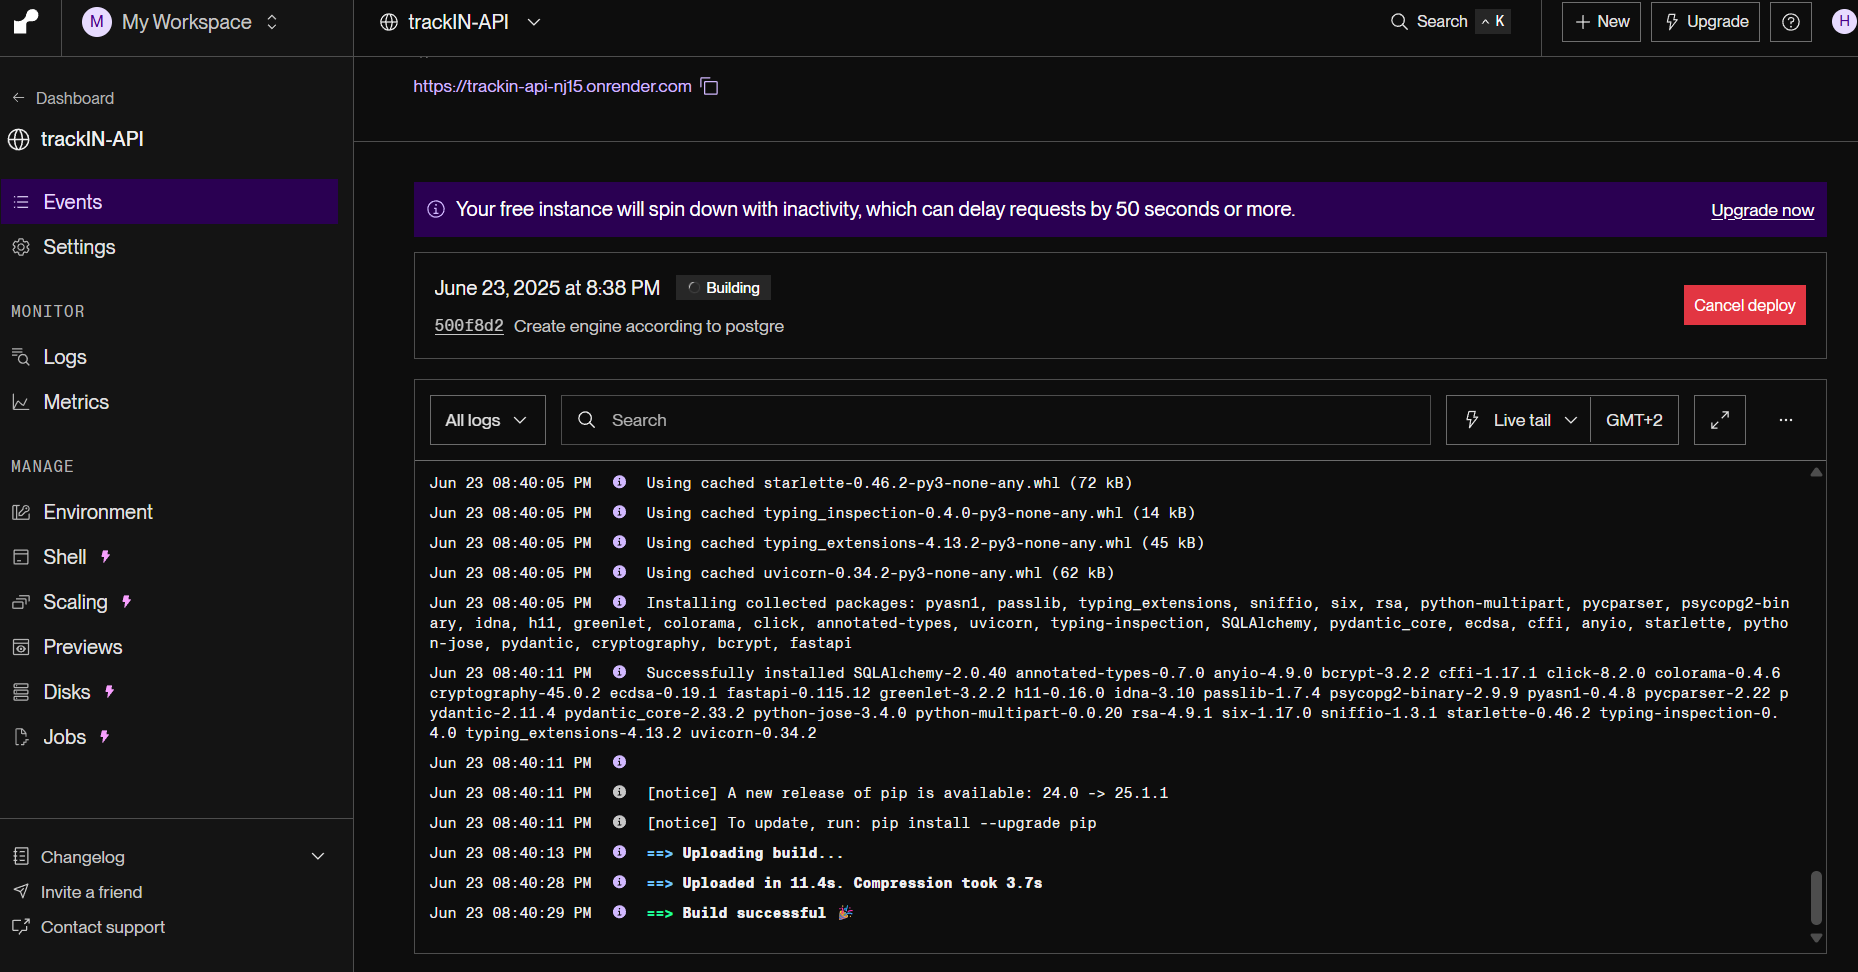
\includegraphics[width=\textwidth]{Project_Screenshots/API.png}
    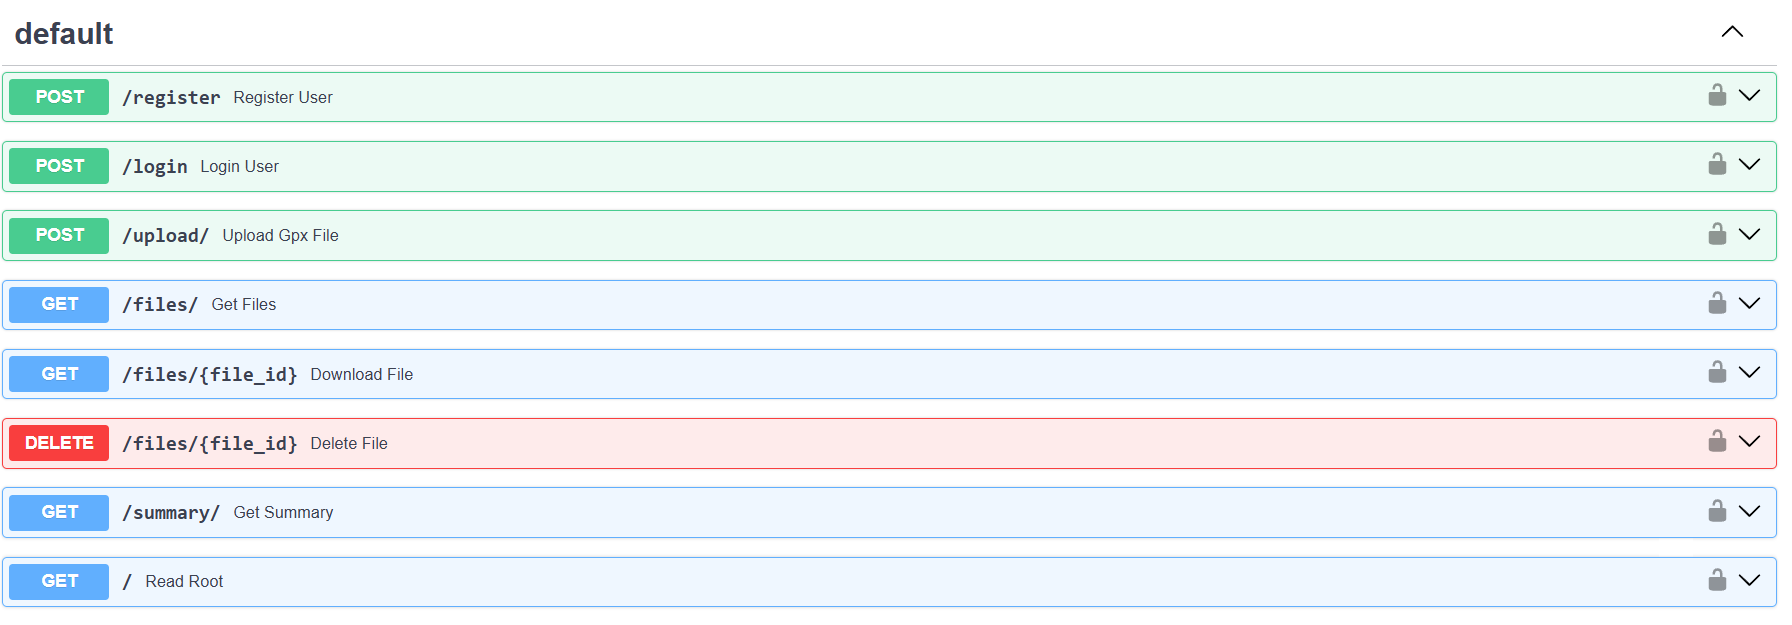
\includegraphics[width=\textwidth]{Project_Screenshots/API2.png}
    \caption{API and framework server }
\end{figure}


\section{Frontend Testing}
\newpage
This document outlines the test protocol for the iOS version of the TrackIN app. The goal is to validate the app’s user interface, functionality, data handling, error recovery, performance, and plotting methods.

\begin{tabular}{ll}
\textbf{Project:} & TrackIN \\
\textbf{Platform:} & iOS \\
\textbf{Version:} & [18.5] \\
\textbf{Tester:} & [Baatarbileg] \\
\textbf{Date:} & June 2025 \\
\end{tabular}

\subsection{User Interface Tests}
\begin{longtable}{|p{2.2cm}|p{5.2cm}|p{4cm}|p{2.5cm}|}
\hline
\textbf{Test Case ID} & \textbf{Description} & \textbf{Expected Result} & \textbf{Status / Notes} \\
\hline
UI-01 & Launch the app & Splash → Home screen appears & Pass \\
\hline
UI-02 & Tap "Start" button & Starts tracking location/time & Pass \\
\hline
UI-03 & Tap "Stop \& GPX" button & Prompt to save/export GPX & Pass \\
\hline
UI-04 & Toggle dark/light mode & UI adjusts without layout issues & Pass \\
\hline
UI-05 & Rotate device & UI adapts to orientation & Pass \\
\hline
\end{longtable}

\subsection{Functionality Tests}
\begin{longtable}{|p{2.2cm}|p{5.2cm}|p{4cm}|p{2.5cm}|}
\hline
\textbf{Test Case ID} & \textbf{Description} & \textbf{Expected Result} & \textbf{Status / Notes} \\
\hline
FUNC-01 & Start and end tracking session & GPX file is saved/shared & Pass \\
\hline
FUNC-02 & Track while moving & Distance and altitude increase & Pass \\
\hline
FUNC-03 & Stop without starting & No effect or show error & Pass \\
\hline
FUNC-04 & Export GPX file & GPX exported with valid XML & Pass \\
\hline
FUNC-05 & Import and view GPX file & Points/elevation shown on map & Needs Fix – file empty \\
\hline
\end{longtable}

\subsection{Data Management Tests}
\begin{longtable}{|p{2.2cm}|p{5.2cm}|p{4cm}|p{2.5cm}|}
\hline
\textbf{Test Case ID} & \textbf{Description} & \textbf{Expected Result} & \textbf{Status / Notes} \\
\hline
DATA-01 & Altitude recording accuracy & Altitude changes recorded accurately & Pass \\
\hline
DATA-02 & Distance recording accuracy & Distance increases with movement & Needs Check \\
\hline
DATA-03 & Simulate GPS noise & App filters or interpolates properly & Needs Work \\
\hline
DATA-04 & Timestamp consistency & All points timestamped correctly & Pass \\
\hline
DATA-05 & GPX XML format validation & XML well-formed and valid & Needs Fix – remove namespace \\
\hline
\end{longtable}

\subsection{Error Handling Tests}
\begin{longtable}{|p{2.2cm}|p{5.2cm}|p{4cm}|p{2.5cm}|}
\hline
\textbf{Test Case ID} & \textbf{Description} & \textbf{Expected Result} & \textbf{Status / Notes} \\
\hline
ERR-01 & Disable location permission & App requests permission or shows error & Pass \\
\hline
ERR-02 & Airplane mode during tracking & Show GPS error or no signal warning & Pass \\
\hline
ERR-03 & Kill app during session & App resumes or informs session loss & Pass – New session starts \\
\hline
ERR-04 & Deny file write permission & Error shown; app remains stable & Pass \\
\hline
\end{longtable}

\subsection{Performance Tests}
\begin{longtable}{|p{2.2cm}|p{5.2cm}|p{4cm}|p{2.5cm}|}
\hline
\textbf{Test Case ID} & \textbf{Description} & \textbf{Expected Result} & \textbf{Status / Notes} \\
\hline
PERF-01 & Run app for 30+ minutes & No crash or memory leak & Pass \\
\hline
PERF-02 & Background tracking & Tracks data when screen is off & Pass \\
\hline
\end{longtable}

\subsection{Plotting Method Tests}
\begin{longtable}{|p{2.2cm}|p{5.2cm}|p{4cm}|p{2.5cm}|}
\hline
\textbf{Test Case ID} & \textbf{Description} & \textbf{Expected Result} & \textbf{Status / Notes} \\
\hline
PLOT-01 & Spline interpolation & Smooth elevation graph & Needs Fix – sudden peaks \\
\hline
PLOT-02 & Loess interpolation (v2) & Smooth and stable plot & Pass \\
\hline
\end{longtable}

The iOS app passes the majority of test cases across UI, functionality, error handling, and performance. Improvements are recommended in data smoothing, GPX importing, and XML formatting. Code coverage testing is enabled and will guide future test improvements.

\begin{figure}[h!]
    \centering
    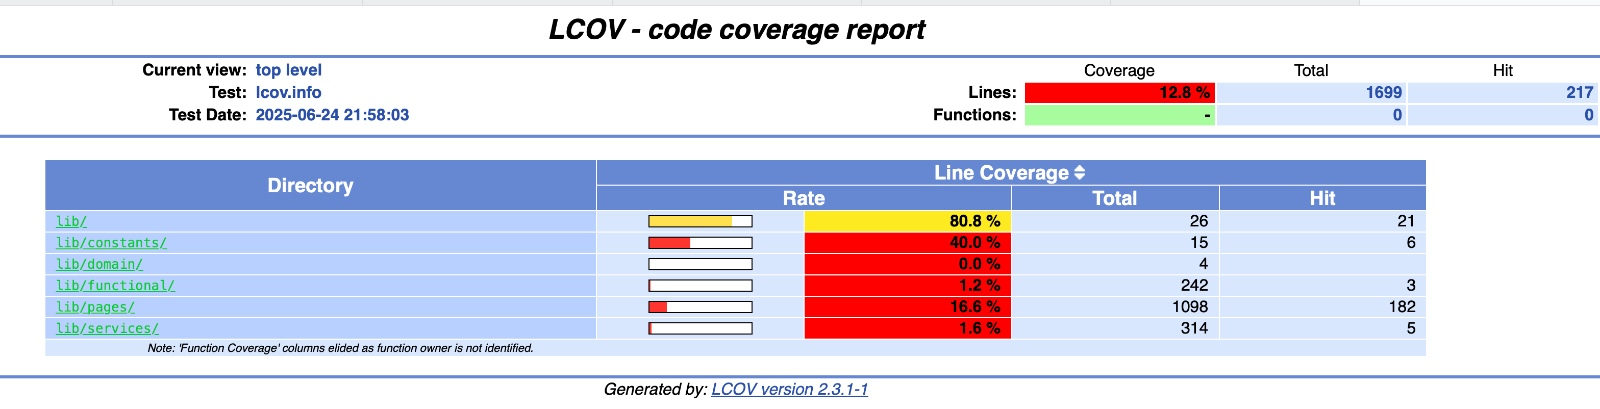
\includegraphics[width=1\textwidth]{Project_Screenshots/coverage1.jpg}
    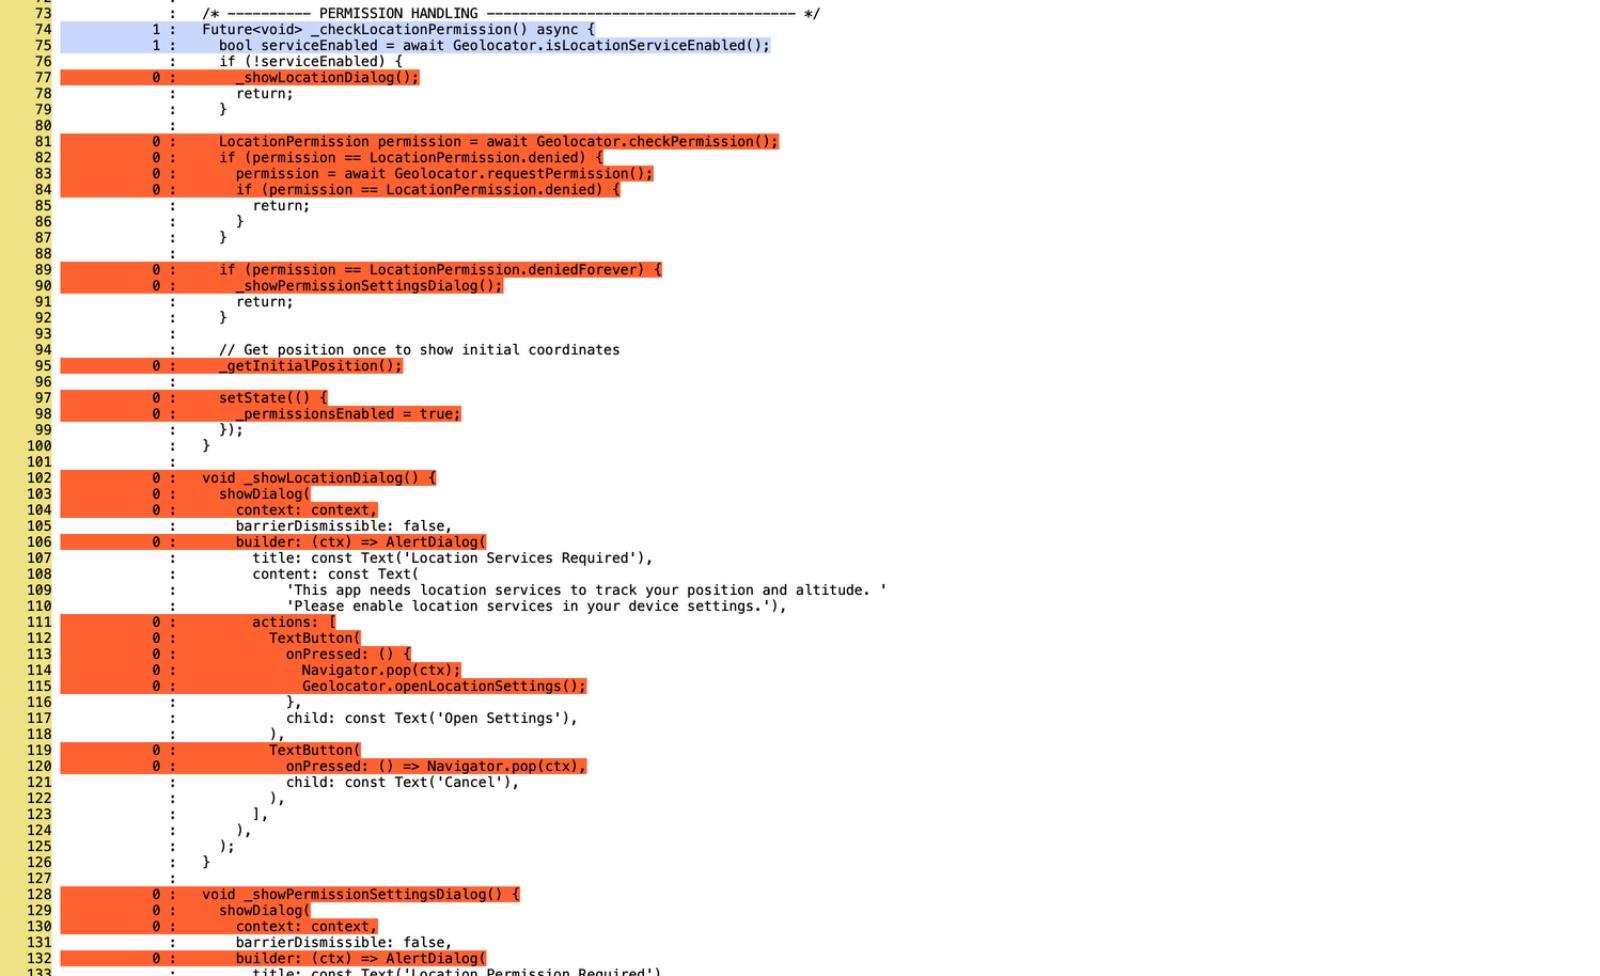
\includegraphics[width=1.5\textwidth]{Project_Screenshots/coverage2.jpg}
    \caption{Coverage test for iOS}
\end{figure}

\vspace{0.5em}
\noindent Overall coverage testing had 12.8\% usage: out of 1699 lines of code, 217 lines were hit.

\section{Backend Testing}

\subsection{Plotter Class Testing (\texttt{test\_plotter.py})}

This document outlines the comprehensive testing strategy applied to the Plotter class within \texttt{plotter.py}. The tests leverage \texttt{pytest} for its testing framework and \texttt{unittest.mock} for effective mocking, ensuring thorough validation of the Plotter's functionality without actual graphical rendering.

\subsubsection*{1. Mocking Strategy (\texttt{mock\_matplotlib} Fixture)}
The \texttt{mock\_matplotlib} fixture is a cornerstone of this test suite, designed to isolate the Plotter class's logic from \texttt{matplotlib}'s graphical output.

\textbf{Purpose:} To prevent \texttt{matplotlib} from opening actual plot windows during test execution. This significantly speeds up tests, eliminates reliance on a display environment, and makes the test suite suitable for continuous integration (CI) pipelines.

\textbf{Implementation Details:}
\begin{itemize}
  \item It uses \texttt{patch('plotter.plt')} to replace the \texttt{matplotlib.pyplot} object (aliased as \texttt{plt} in \texttt{plotter.py}) with a \texttt{MagicMock}.
  \item Crucially, it simulates the \texttt{matplotlib} object hierarchy:
  \begin{itemize}
    \item \texttt{mock\_plt.figure.return\_value = mock\_fig}: Ensures that when \texttt{plt.figure()} is called, it returns a mock figure object (\texttt{mock\_fig}).
    \item \texttt{mock\_fig.add\_subplot.return\_value = mock\_ax}: Configures \texttt{mock\_fig} so that calling \texttt{add\_subplot()} on it returns a mock axes object (\texttt{mock\_ax}).
  \end{itemize}
  \item \textbf{Explicit Mocking:} Key \texttt{matplotlib.pyplot} functions (\texttt{plot}, \texttt{title}, \texttt{xlabel}, \texttt{show}, etc.) and \texttt{matplotlib.axes} methods (\texttt{plot}, \texttt{set\_title}, etc.) that \texttt{Plotter} directly calls are individually mocked using \texttt{MagicMock()}.
\end{itemize}

\textbf{Benefit:} Enables tests to verify what \texttt{matplotlib} functions are called and with what arguments, rather than attempting to validate visual output.

\subsubsection*{2. Dummy Data Fixtures}
To ensure self-contained and repeatable tests, controlled dummy data is used.

\begin{itemize}
  \item \textbf{\texttt{dummy\_elevation\_profile}:} Provides a basic, valid \texttt{ElevationProfile} instance created with a list of \texttt{Point} objects.
  \item \textbf{\texttt{another\_dummy\_elevation\_profile}:} Supplies a second, distinct \texttt{ElevationProfile} with different (but similarly structured) point data.
\end{itemize}

\subsubsection*{3. Test Cases (\texttt{TestPlotter} Class)}
The \texttt{TestPlotter} class is structured to systematically test each component of the \texttt{Plotter} class.

\paragraph{a. Initialization Tests (\texttt{test\_init\_*})}
\begin{itemize}
  \item \texttt{test\_init\_no\_profiles}: Initializes \texttt{Plotter} without any profiles. Verifies \texttt{plotter.profiles} is empty.
  \item \texttt{test\_init\_with\_single\_profile\_auto\_named}: Adds one \texttt{ElevationProfile} without a name. Profile is auto-named \texttt{"Profile 1"}.
  \item \texttt{test\_init\_with\_single\_profile\_named}: Adds one profile with a given name.
  \item \texttt{test\_init\_with\_single\_profile\_named\_none}: Name is \texttt{None} \textrightarrow{} auto-named \texttt{"Profile 1"}. (Edge Case)
  \item \texttt{test\_init\_with\_multiple\_profiles\_auto\_named}: Adds multiple unnamed profiles \textrightarrow{} named sequentially.
  \item \texttt{test\_init\_with\_multiple\_profiles\_mixed\_names}: Mix of named and unnamed profiles added correctly.
\end{itemize}

\paragraph{b. Unique Name Generation Tests (\texttt{\_generate\_unique\_name})}
\begin{itemize}
  \item \texttt{test\_generate\_unique\_name\_empty}: Returns \texttt{"Profile 1"} when no profiles exist.
  \item \texttt{test\_generate\_unique\_name\_existing}: Returns \texttt{"Profile 2"} when \texttt{"Profile 1"} exists.
  \item \texttt{test\_generate\_unique\_name\_with\_gap}: Handles skipped names like \texttt{"Profile 1"} and \texttt{"Profile 3"} \textrightarrow{} returns \texttt{"Profile 2"} (Edge Case).
\end{itemize}

\paragraph{c. Adding Profiles Tests (\texttt{add\_profiles})}
\begin{itemize}
  \item \texttt{test\_add\_profiles\_single\_auto\_name}: Adds unnamed profile \textrightarrow{} auto-named.
  \item \texttt{test\_add\_profiles\_single\_named}: Adds named profile.
  \item \texttt{test\_add\_profiles\_multiple\_named}: Adds multiple named profiles.
  \item \texttt{test\_add\_profiles\_mixed\_input}: Mix of named and unnamed profiles in one call.
  \item \texttt{test\_add\_profiles\_duplicate\_name\_overwrites}: Duplicate name replaces old one (Edge Case).
  \item \texttt{test\_add\_profiles\_empty\_string\_name\_auto\_named}: Empty string name \textrightarrow{} auto-named (Edge Case).
  \item \texttt{test\_add\_profiles\_none\_name\_auto\_named}: \texttt{None} as name \textrightarrow{} auto-named (Edge Case).
  \item \texttt{test\_add\_profiles\_invalid\_input}: Invalid inputs raise \texttt{ValueError} (Edge Case).
\end{itemize}

\paragraph{d. Setting Profiles Tests (\texttt{set\_profiles})}
\begin{itemize}
  \item \texttt{test\_set\_profiles\_valid}: Replaces profiles with valid dict.
  \item \texttt{test\_set\_profiles\_empty\_dict}: Clears all profiles (Edge Case).
  \item \texttt{test\_set\_profiles\_invalid\_type}: Non-dict input \textrightarrow{} \texttt{TypeError} (Edge Case).
  \item \texttt{test\_set\_profiles\_invalid\_value}: Invalid value types \textrightarrow{} \texttt{ValueError} (Edge Case).
\end{itemize}

\paragraph{e. Plotting Method Tests}
\begin{itemize}
  \item \texttt{test\_*\_no\_profiles}: No profiles \textrightarrow{} "No profiles to plot." printed; no matplotlib functions called (Edge Case).
  \item \texttt{test\_plot\_distance\_vs\_elevation\_single\_profile}: Single profile, custom title/labels \textrightarrow{} all plot functions called once.
  \item \texttt{test\_plot\_distance\_vs\_elevation\_multiple\_profiles}: Multiple profiles \textrightarrow{} verify plot call count and arguments.
  \item \texttt{test\_plot\_3d\_lat\_lon\_elevation\_single\_profile}: 3D plot for single profile \textrightarrow{} verify projection, labels, and plot call.
  \item \texttt{test\_plot\_3d\_lat\_lon\_elevation\_multiple\_profiles}: Multiple 3D profiles \textrightarrow{} verify correct call sequence for each.
\end{itemize}

\textbf{Conclusion:} This detailed testing approach ensures the \texttt{Plotter} class is robust, handles various valid and invalid inputs gracefully, and correctly interacts with its \texttt{matplotlib} dependency via mock objects.


\subsection{Model Classes Testing (\texttt{test\_models.py})}

This document outlines the testing strategy, covered functionalities, and specific edge cases addressed in the \texttt{test\_models.py} file. The primary goal of these tests is to ensure the robust and correct behavior of the \texttt{Point}, \texttt{ElevationProfile}, and \texttt{Track} classes defined in \texttt{models.py}.

\subsubsection*{1. Introduction}
\texttt{test\_models.py} contains unit tests designed to verify the core data structures used throughout the GPX data processing application. These tests are isolated from external dependencies wherever possible through the use of mocking, ensuring fast, reliable, and repeatable execution.

\subsubsection*{2. Tests for the \texttt{Point} Class}
\begin{itemize}
  \item \texttt{test\_point\_init\_with\_elevation}: Verifies initialization with latitude, longitude, and elevation.
  \item \texttt{test\_point\_init\_without\_elevation}: Elevation defaults to \texttt{None} if not provided.
  \item \texttt{test\_point\_to\_dict\_with\_elevation} / \texttt{without\_elevation}: Checks dictionary output depending on elevation presence.
  \item \texttt{test\_point\_haversine\_distance\_identical\_points}: Ensures distance between identical points is 0.
  \item \texttt{test\_point\_haversine\_distance\_known\_values}: Verifies correct distance computation with known locations using \texttt{pytest.approx}.
  \item \texttt{test\_point\_distance\_to}: Ensures \texttt{distance\_to()} internally calls static \texttt{haversine\_distance()} (mocked).
  \item \texttt{test\_point\_copy}: Confirms \texttt{copy()} produces a new object with same values.
\end{itemize}

\subsubsection*{3. Tests for the \texttt{ElevationProfile} Class}
\begin{itemize}
  \item Initialization:
  \begin{itemize}
    \item \texttt{test\_elevation\_profile\_init\_empty\_list}, \texttt{single\_point}, \texttt{multiple\_points}
    \item For multiple points, cumulative distances are verified with mocked \texttt{Point.haversine\_distance}.
  \end{itemize}
  \item Accessors:
  \begin{itemize}
    \item \texttt{get\_latitudes}, \texttt{get\_longitudes}, \texttt{get\_elevations}, \texttt{get\_distances}
  \end{itemize}
  \item Mutators:
  \begin{itemize}
    \item \texttt{set\_elevations\_valid}, \texttt{with\_none\_values}, \texttt{empty\_list}, \texttt{length\_mismatch}
  \end{itemize}
  \item Statistics:
  \begin{itemize}
    \item \texttt{get\_elevation\_stats\_normal\_case}\newline
    \texttt{get\_elevation\_stats\_with\_none\_elevations\_...}: Highlights a known \texttt{TypeError} bug with \texttt{None} values.
    \item \texttt{get\_elevation\_stats\_empty\_profile}, \texttt{all\_none\_elevations}, \texttt{single\_point}
  \end{itemize}
  \item \texttt{test\_elevation\_profile\_copy}: Verifies deep copying of profiles.
\end{itemize}

\subsubsection*{4. Tests for the \texttt{Track} Class}
\textbf{Focus:} The \texttt{from\_gpx\_file} factory method using mocked I/O and external dependencies.

\textbf{Mocking Strategy:}
\begin{itemize}
  \item \texttt{patch('builtins.open', mock\_open(...))}: Prevents file I/O, supplies dummy GPX.
  \item \texttt{patch('gpxpy.parse')} returns a mocked GPX object.
  \item Mocked internal GPX hierarchy: \texttt{tracks}, \texttt{segments}, \texttt{points}.
  \item \texttt{patch('models.GeoidKarney')} returns 0.0 when called as function.
  \item \texttt{patch('pygeodesy.ellipsoidalKarney.LatLon')} returns mock \texttt{LatLon}.
  \item \texttt{patch.object(Point, 'haversine\_distance')} and \texttt{distance\_to} mocked to return 1.0.
\end{itemize}

\textbf{Track Test Cases:}
\begin{itemize}
  \item \texttt{test\_track\_from\_gpx\_file\_valid\_data}: Creates \texttt{Track} with points + elevations.
  \item \texttt{test\_track\_from\_gpx\_file\_no\_elevation\_data}: Expects \texttt{TypeError} on \texttt{None} elevation (known issue).
  \item \texttt{test\_track\_from\_gpx\_file\_empty\_gpx\_object}: Yields an empty \texttt{Track}.
  \item \texttt{test\_track\_from\_gpx\_file\_gpx\_parse\_exception}: Simulates parse error \textrightarrow{} raises \texttt{ValueError}.
  \item \texttt{test\_track\_from\_gpx\_file\_multiple\_tracks\_and\_segments}: Verifies correct point concatenation.
\end{itemize}

\subsubsection*{5. Testing Practices Used}
\begin{itemize}
  \item \texttt{pytest} for discovery, assertion, and execution.
  \item \texttt{unittest.mock}: Extensive use of \texttt{patch}, \texttt{MagicMock}, \texttt{mock\_open}.
  \item \texttt{pytest.approx}: Used for floating-point tolerance.
  \item Clear assertion patterns: \texttt{assert}, \texttt{pytest.raises}, equality checks.
\end{itemize}

\subsubsection*{6. Conclusion and Developer Notes}
All tests in \texttt{test\_models.py} are passing, supporting a reliable data layer.

\textbf{Important Observation:} The following tests reveal a runtime bug:
\begin{itemize}
  \item \texttt{test\_elevation\_profile\_get\_elevation\_stats\_with\_none\_elevations\_...}
  \item \texttt{test\_track\_from\_gpx\_file\_no\_elevation\_data}
\end{itemize}
Both expose that \texttt{None} elevation values cause \texttt{TypeError} in arithmetic.

\textbf{Recommendation:} Modify \texttt{models.py} to gracefully handle \texttt{None} elevations:
\begin{itemize}
  \item Skip or interpolate \texttt{None} values in stats.
  \item Avoid subtracting float from \texttt{None} in \texttt{Track.from\_gpx\_file}.
\end{itemize}
This will improve the system's robustness when handling real-world GPX data with incomplete elevation profiles.

\subsection{Elevation API Testing (\texttt{test\_elevation\_api.py})}

This section documents the unit testing performed on the \texttt{elevation\_api.py} module, which defines two classes: \texttt{ElevationAPI} and \texttt{OpenElevationAPI}. These classes are responsible for retrieving elevation data based on geographic coordinates via external APIs.

\subsubsection*{1. Introduction}
The goal of these tests is to ensure the robustness of both API clients in handling successful responses as well as a wide range of failure scenarios.

\subsubsection*{2. Testing Approach}
All tests use Python's built-in \texttt{unittest} framework. Extensive mocking is employed to isolate logic from actual web API calls.

\textbf{Mocking Strategy:}
\begin{itemize}
  \item \texttt{requests.post} is patched to:
  \begin{itemize}
    \item Prevent real HTTP calls
    \item Return custom mock responses for different scenarios
    \item Simulate exceptions (e.g., \texttt{ConnectionError})
    \item Assert correctness of request URL and payload
  \end{itemize}
  \item \texttt{sys.stdout} is patched using \texttt{io.StringIO} to capture and verify printed error messages.
\end{itemize}

\subsubsection*{3. Tested Components}
\begin{itemize}
  \item \texttt{ElevationAPI.get\_elevations()}
  \item \texttt{OpenElevationAPI.get\_elevations()}
\end{itemize}

\subsubsection*{4. Detailed Test Scenarios}
The following test scenarios and edge cases are implemented for both classes.

\paragraph{4.1 Handling Empty List of Points}
\begin{itemize}
  \item \textbf{Purpose:} Ensure method returns an empty list if input is empty.
  \item \textbf{Behavior:} No API call is made.
\end{itemize}

\paragraph{4.2 Successful API Response}
\begin{itemize}
  \item \textbf{Mocking:} \texttt{requests.post} returns a mocked object with \texttt{ok = True} and valid JSON.
  \item \textbf{Behavior:}
  \begin{itemize}
    \item Parsed elevations match mock data.
    \item Request URL and payload are validated.
  \end{itemize}
\end{itemize}

\paragraph{4.3 HTTP Error Response (4xx/5xx)}
\begin{itemize}
  \item \textbf{Mocking:} \texttt{ok = False}, e.g., status code 404 or 500.
  \item \textbf{Behavior:}
  \begin{itemize}
    \item Returns empty list.
    \item Prints specific API error message to \texttt{stdout}.
  \end{itemize}
\end{itemize}

\paragraph{4.4 Network Connection Error}
\begin{itemize}
  \item \textbf{Mocking:} \texttt{requests.post.side\_effect = ConnectionError("Test error")}
  \item \textbf{Behavior:}
  \begin{itemize}
    \item Returns empty list.
    \item Prints connection error message.
  \end{itemize}
\end{itemize}

\paragraph{4.5 Generic Unexpected Exception}
\begin{itemize}
  \item \textbf{Mocking:} \texttt{side\_effect = Exception("Some unexpected issue")}
  \item \textbf{Behavior:}
  \begin{itemize}
    \item Returns empty list.
    \item Prints "Unexpected error: ..." to \texttt{stdout}.
  \end{itemize}
\end{itemize}

\subsubsection*{5. Conclusion}
All test cases for \texttt{ElevationAPI} and \texttt{OpenElevationAPI} passed successfully. The use of extensive mocking enables fast, reliable testing and confirms that the APIs handle:
\begin{itemize}
  \item Successful responses
  \item API-level HTTP errors
  \item Network failures
  \item Unexpected exceptions
\end{itemize}
This demonstrates that the module is well-prepared for real-world deployment where connectivity and data integrity cannot always be guaranteed.

\begin{figure}[h!]
    \centering
    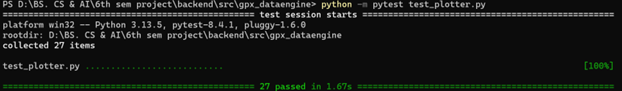
\includegraphics[width=0.95\textwidth]{Project_Screenshots/plotter.png}
   
    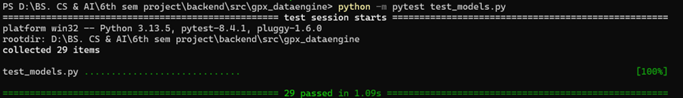
\includegraphics[width=0.95\textwidth]{Project_Screenshots/model.png}

    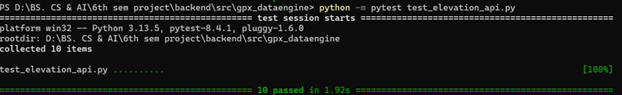
\includegraphics[width=0.95\textwidth]{Project_Screenshots/elevation.png}
    \caption{Execution of each Python test file on terminal to verify passing status.}
    \label{fig:test-py-outputs}
\end{figure}


\clearpage

\newpage
\section{GUI}
\begin{figure}[h!]
    \centering
    % Row 1
    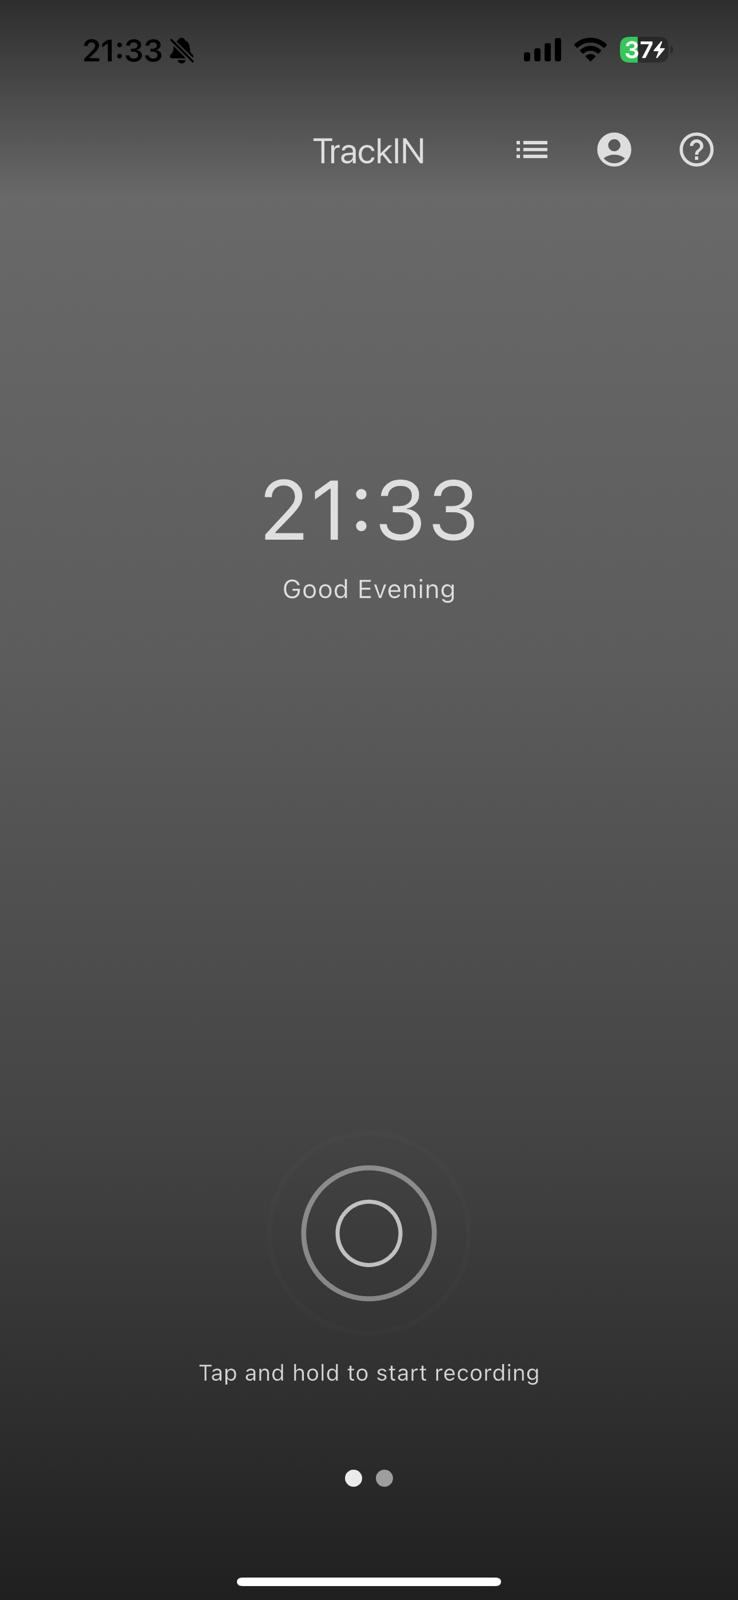
\includegraphics[width=0.23\textwidth]{Project_Screenshots/iOS-1.jpeg}
    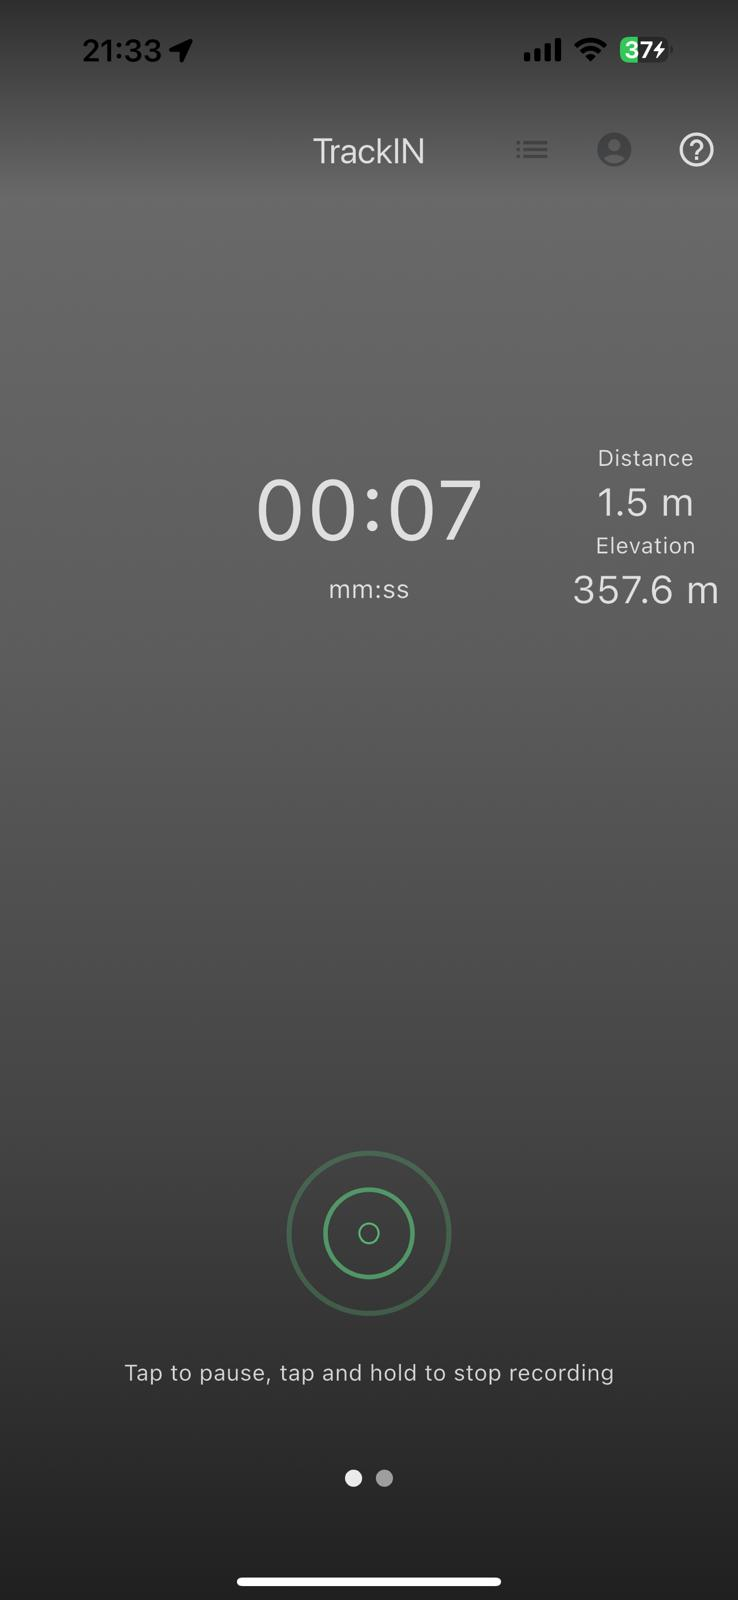
\includegraphics[width=0.23\textwidth]{Project_Screenshots/iOS-2.jpeg}
    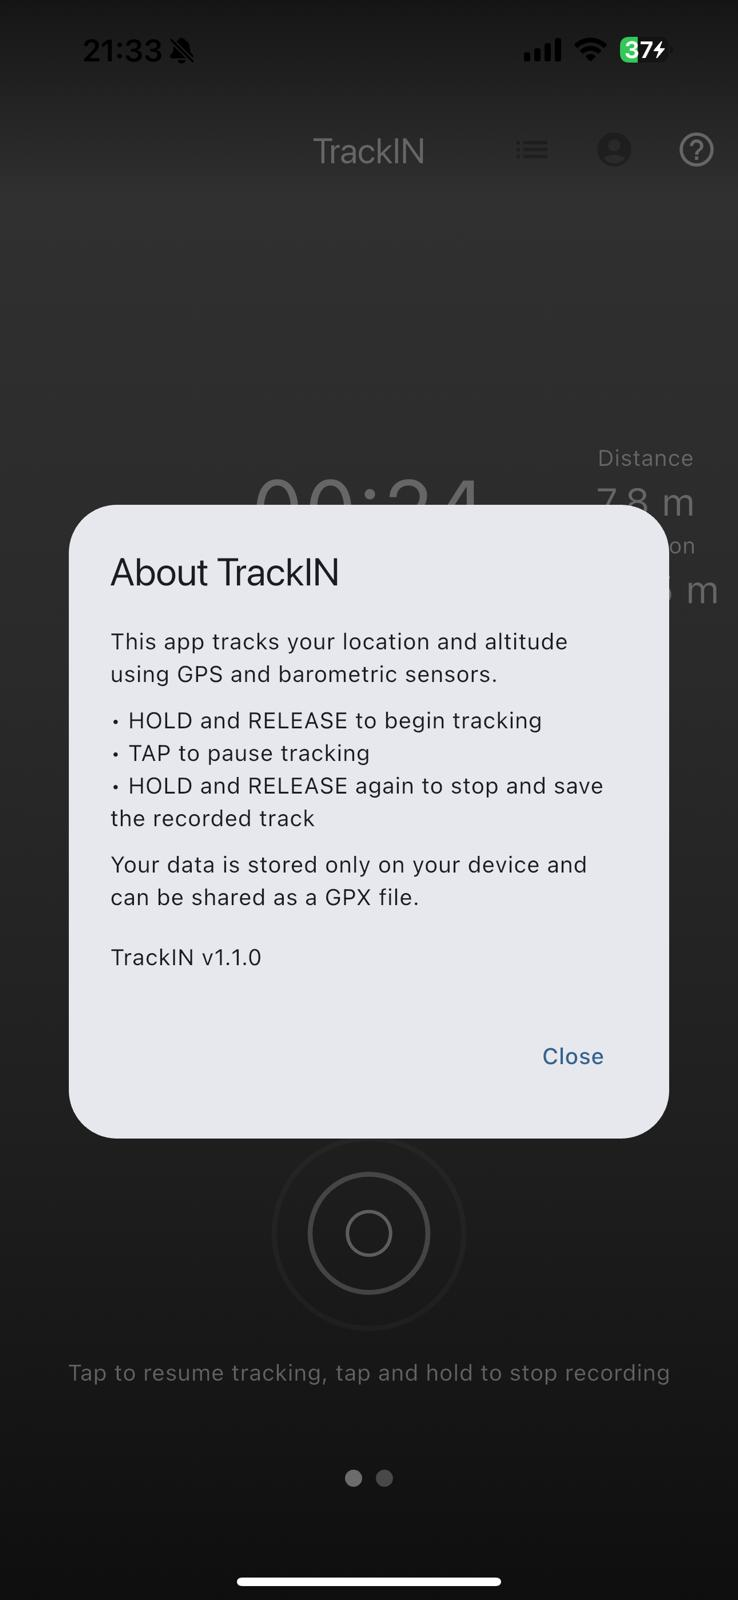
\includegraphics[width=0.23\textwidth]{Project_Screenshots/iOS-3.jpeg}
    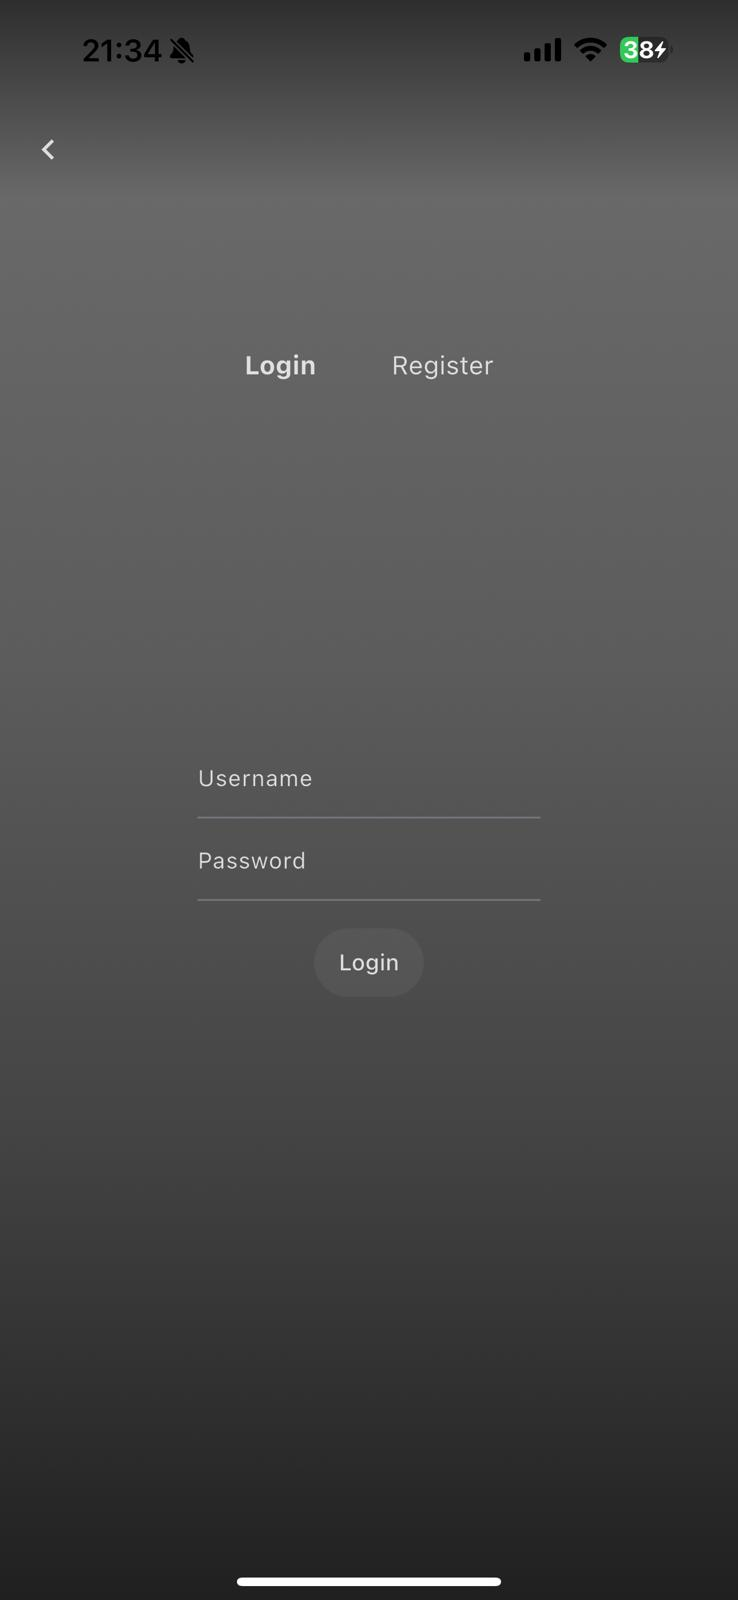
\includegraphics[width=0.23\textwidth]{Project_Screenshots/iOS-4.jpeg}

    \vspace{0.5em} % spacing between rows

    % Row 2
    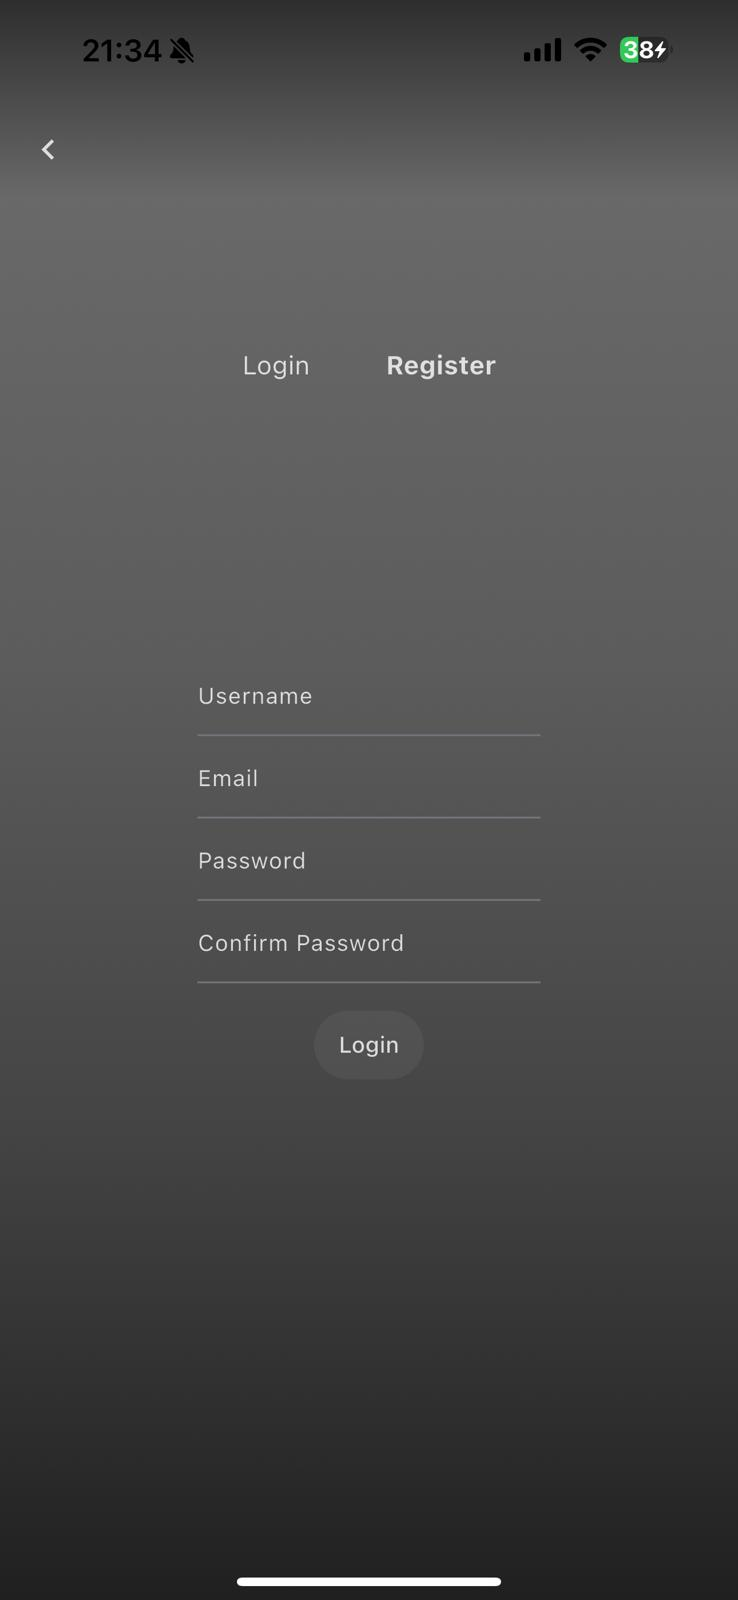
\includegraphics[width=0.23\textwidth]{Project_Screenshots/iOS-5.jpeg}
    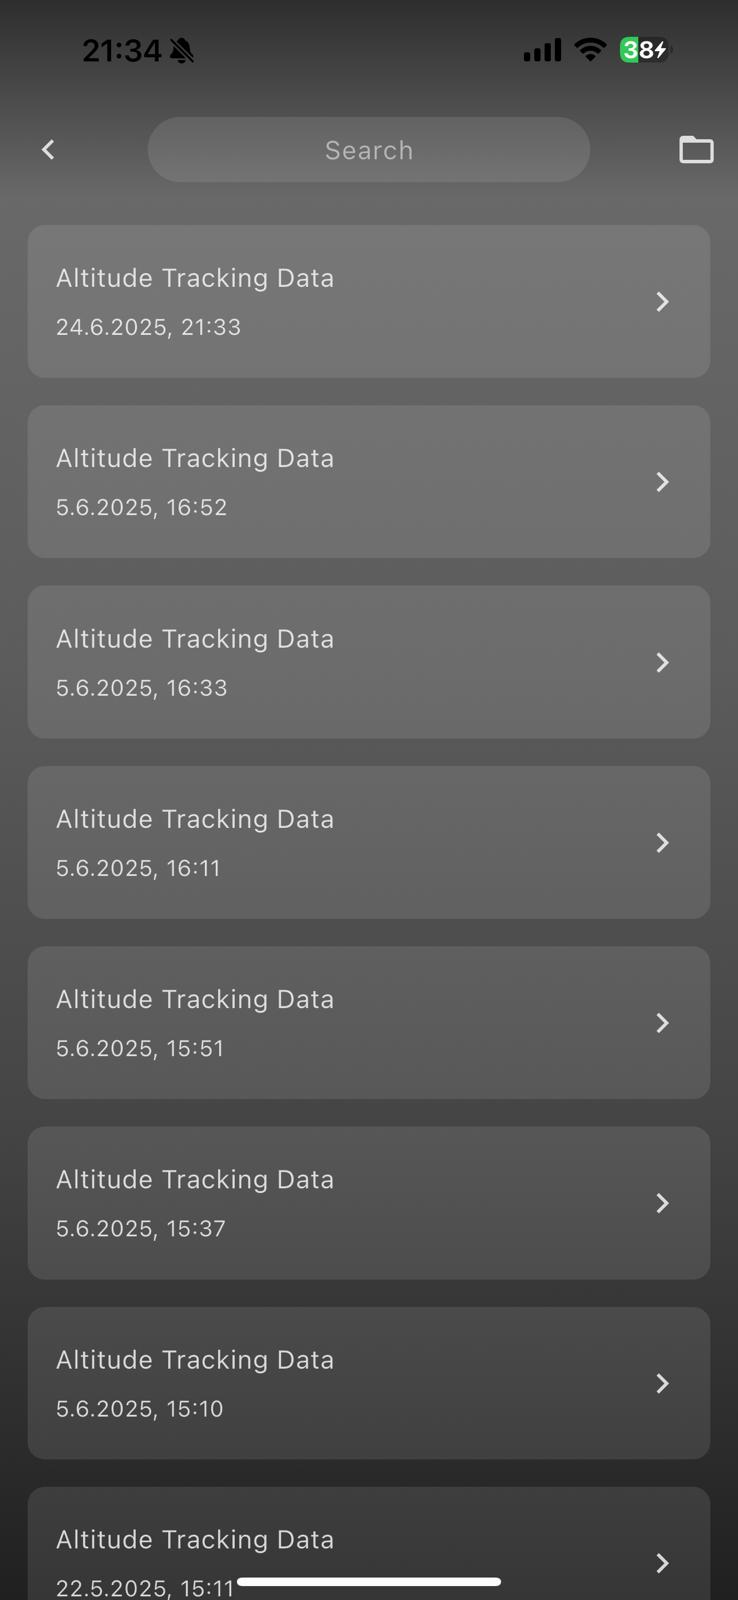
\includegraphics[width=0.23\textwidth]{Project_Screenshots/iOS-6.jpeg}
    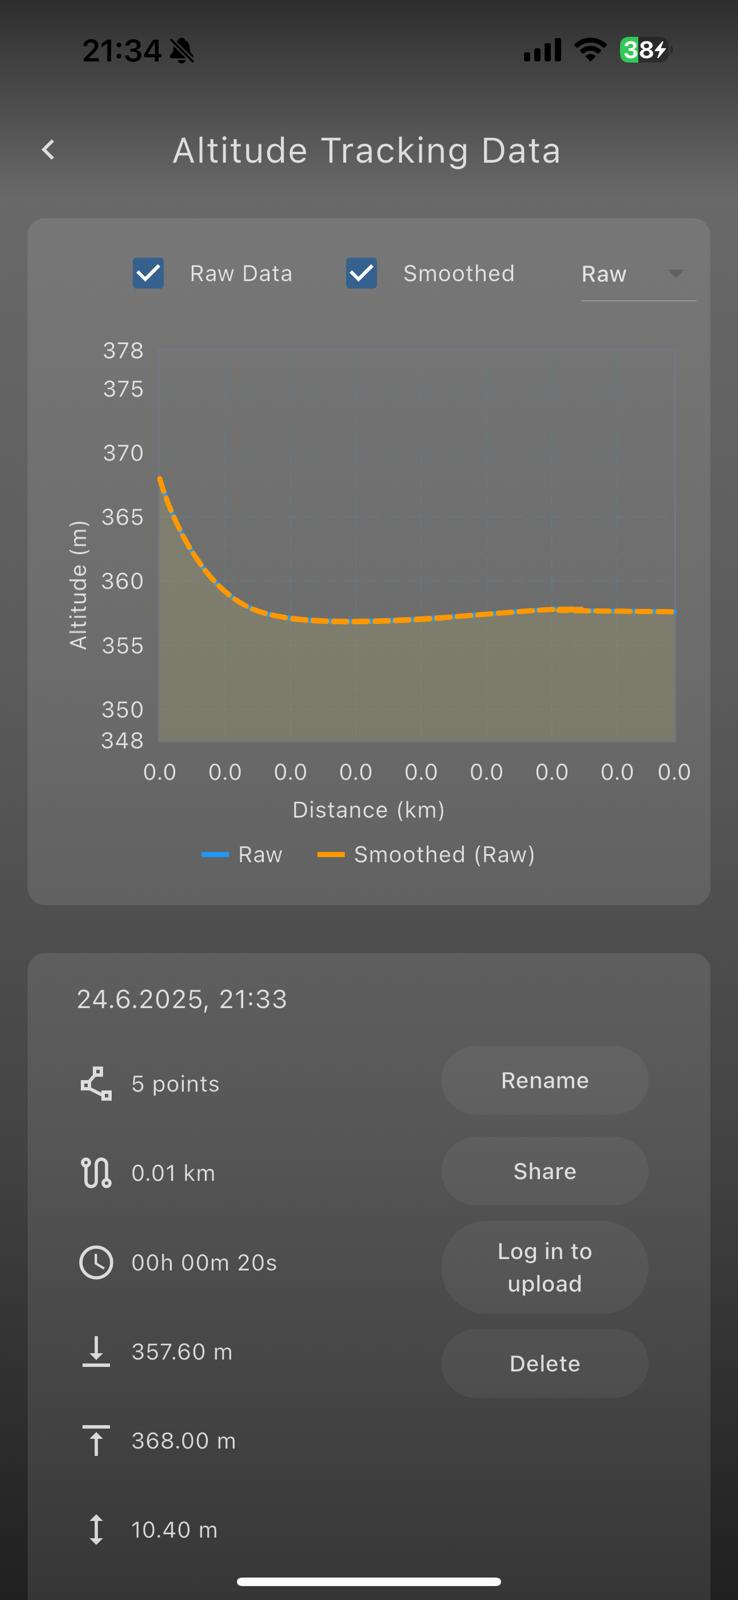
\includegraphics[width=0.23\textwidth]{Project_Screenshots/iOS-7.jpeg}
    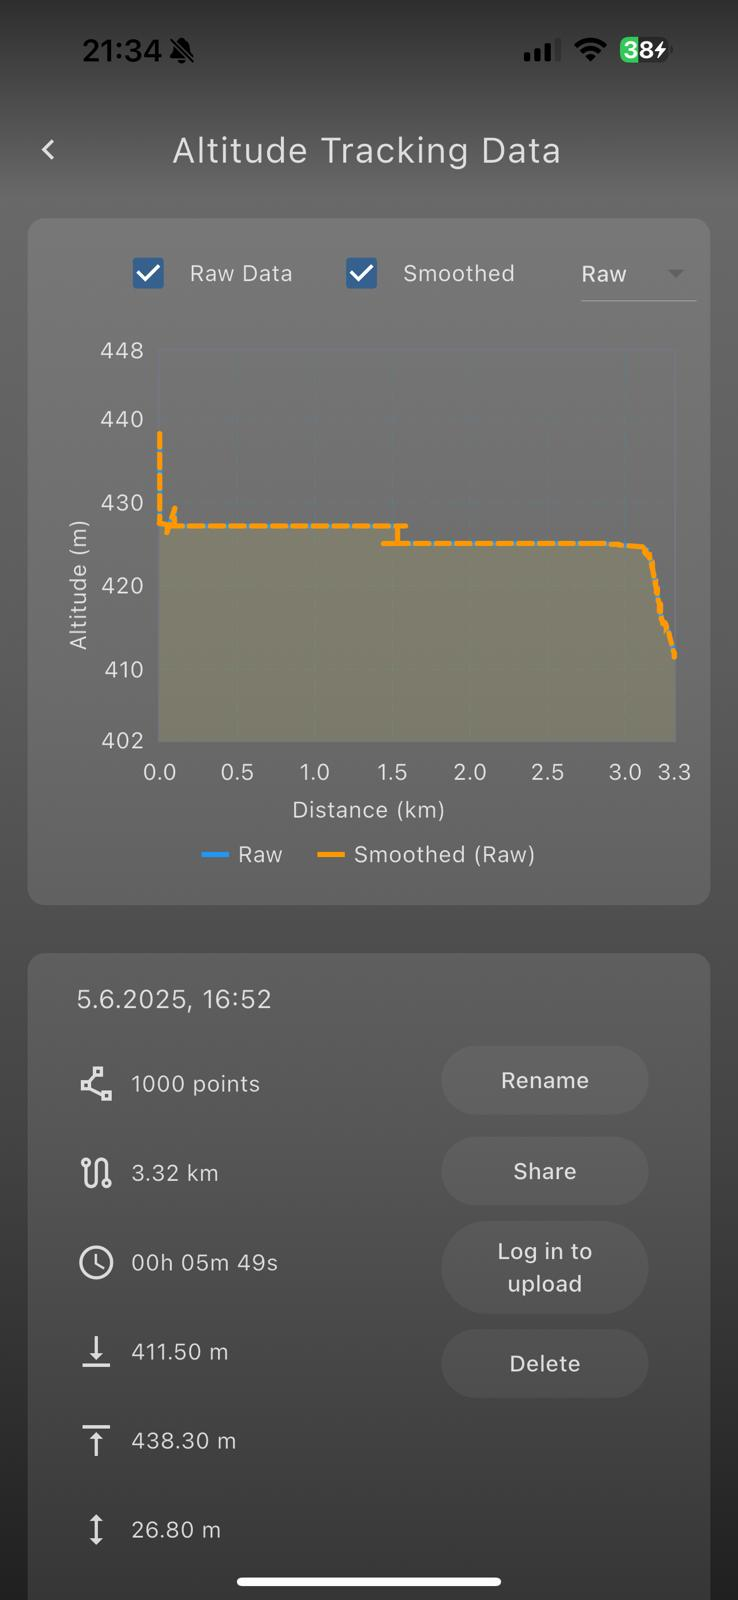
\includegraphics[width=0.23\textwidth]{Project_Screenshots/iOS-8.jpeg}

    \caption{Flutter Application/ iOS and Andriod GUI}
\end{figure}
\begin{figure}[h!]
    \centering
    % Row 1
    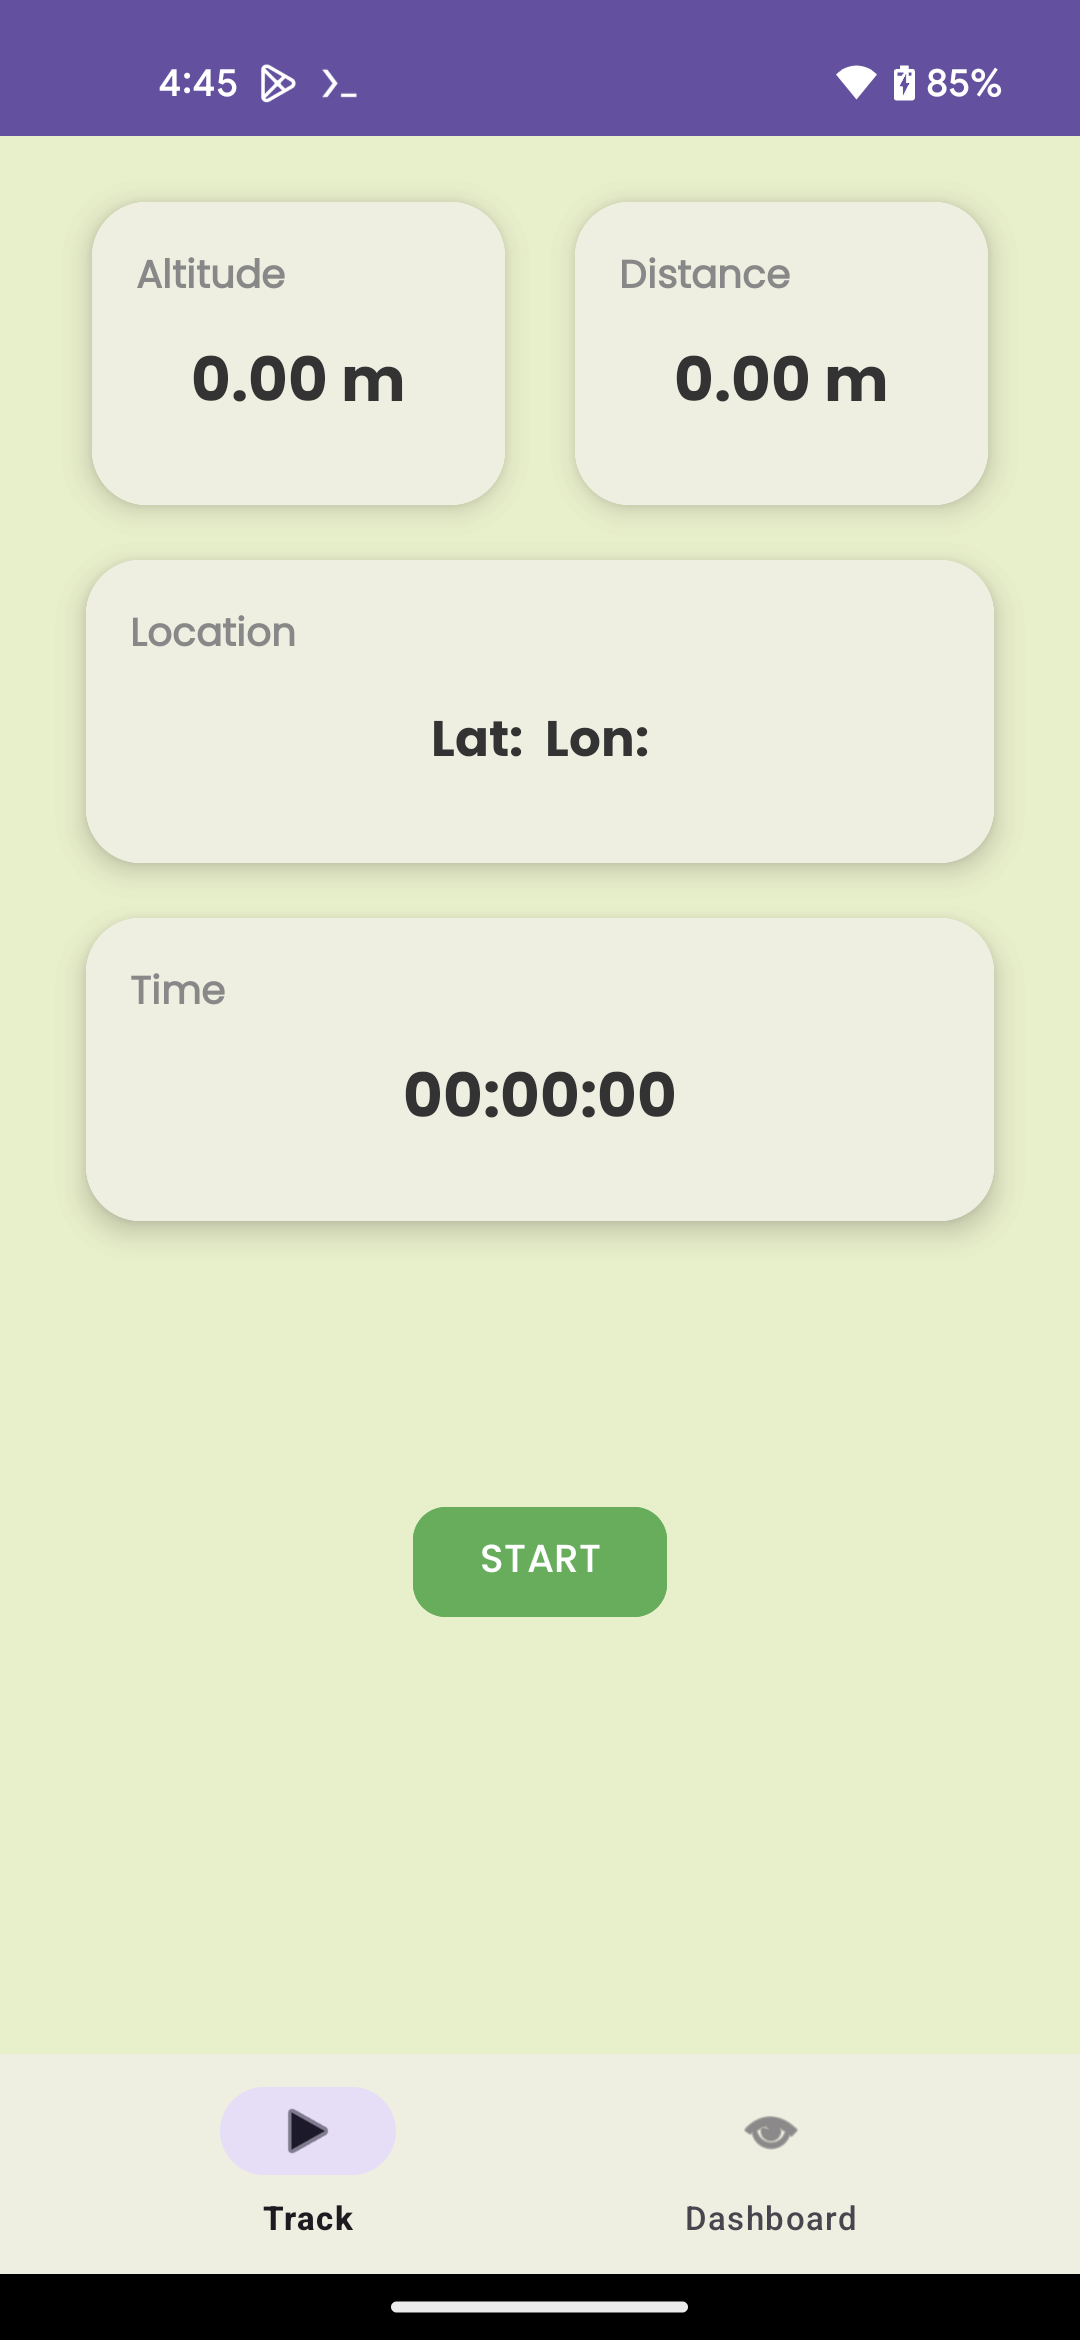
\includegraphics[width=0.23\textwidth]{Project_Screenshots/java1.png}
    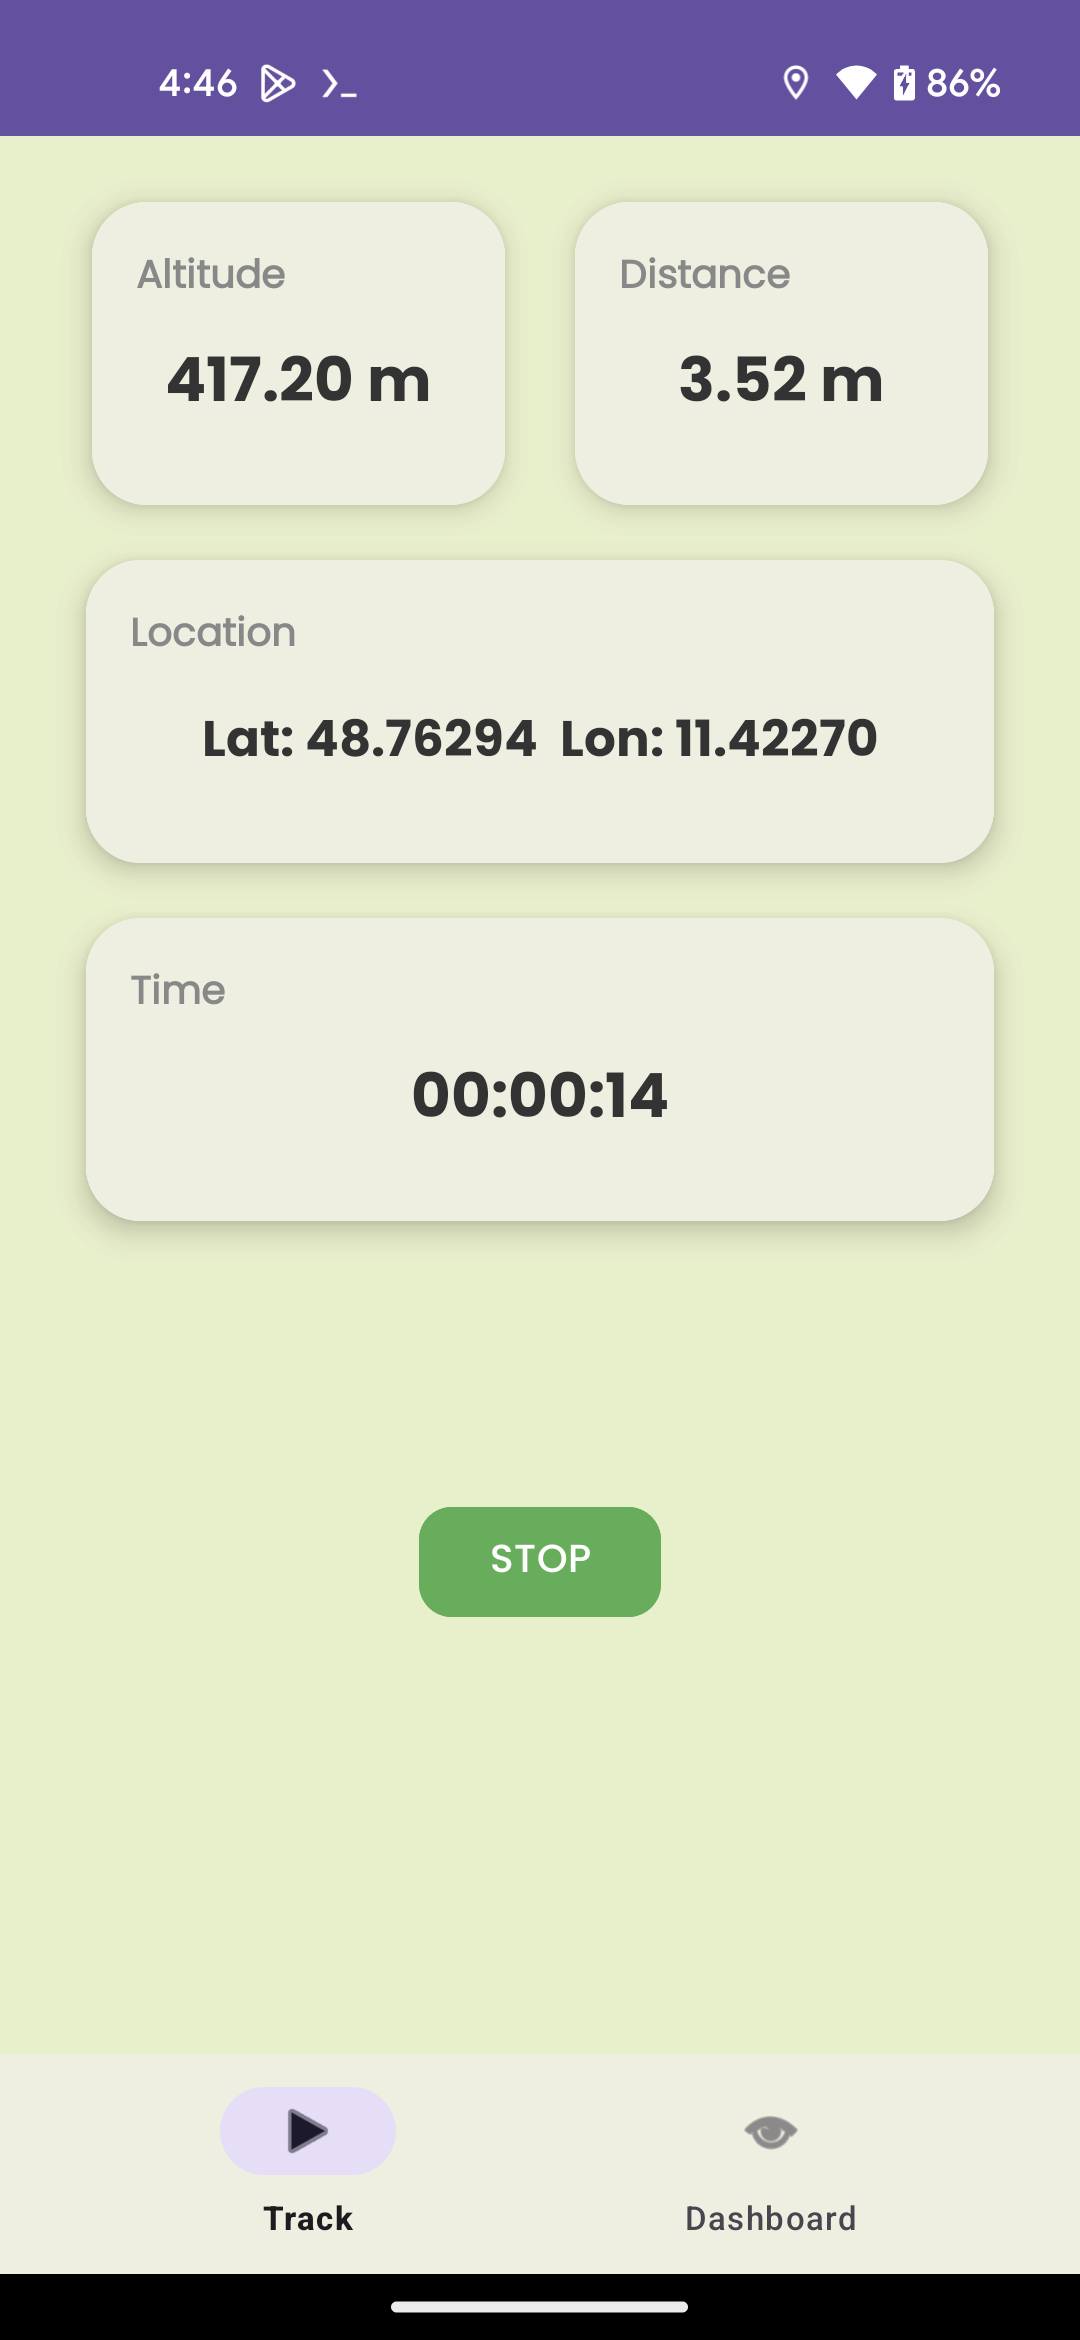
\includegraphics[width=0.23\textwidth]{Project_Screenshots/java2.png}
    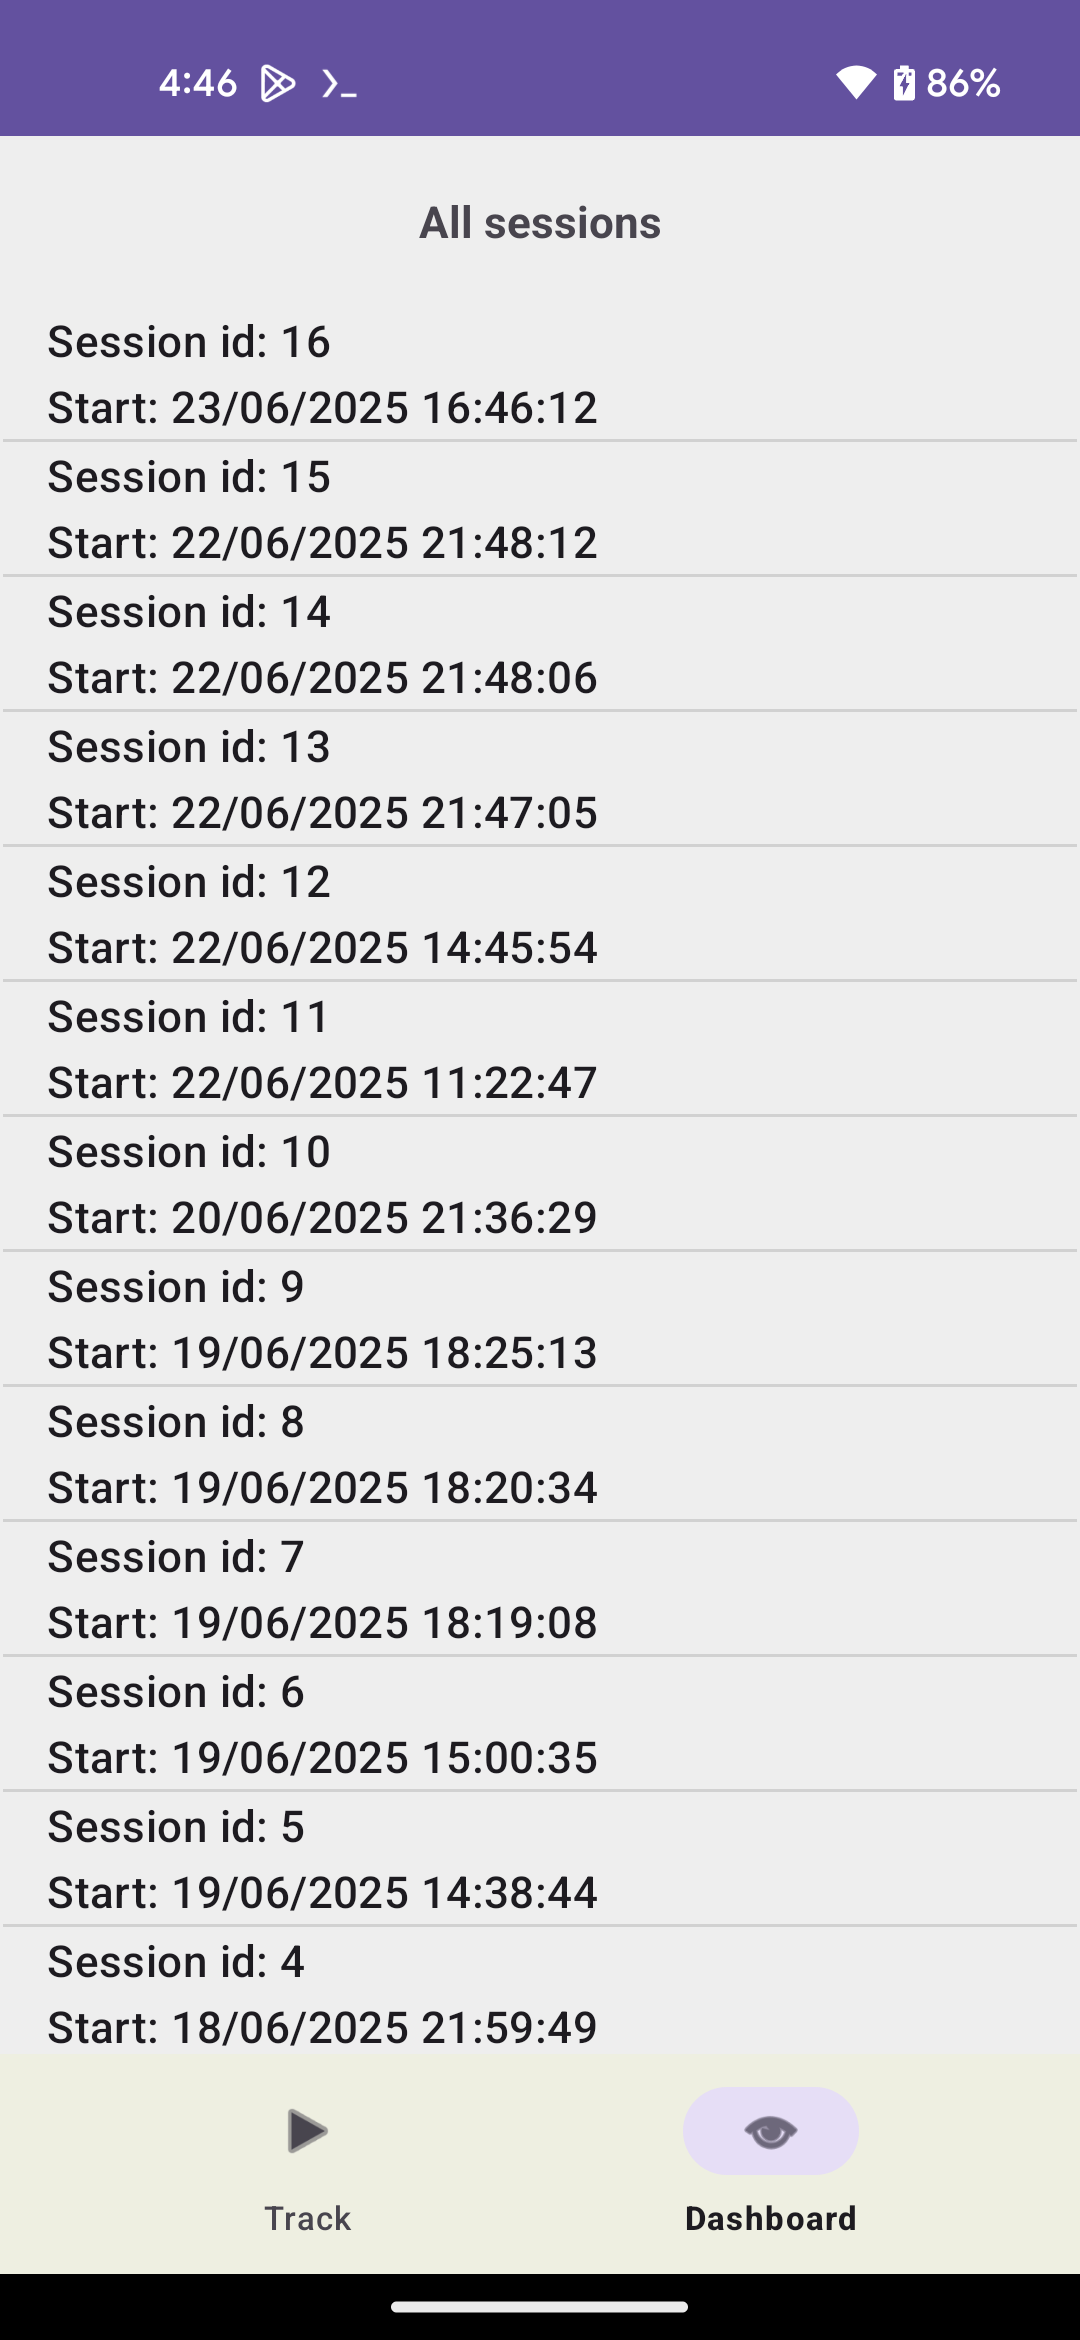
\includegraphics[width=0.23\textwidth]{Project_Screenshots/java3.png}
    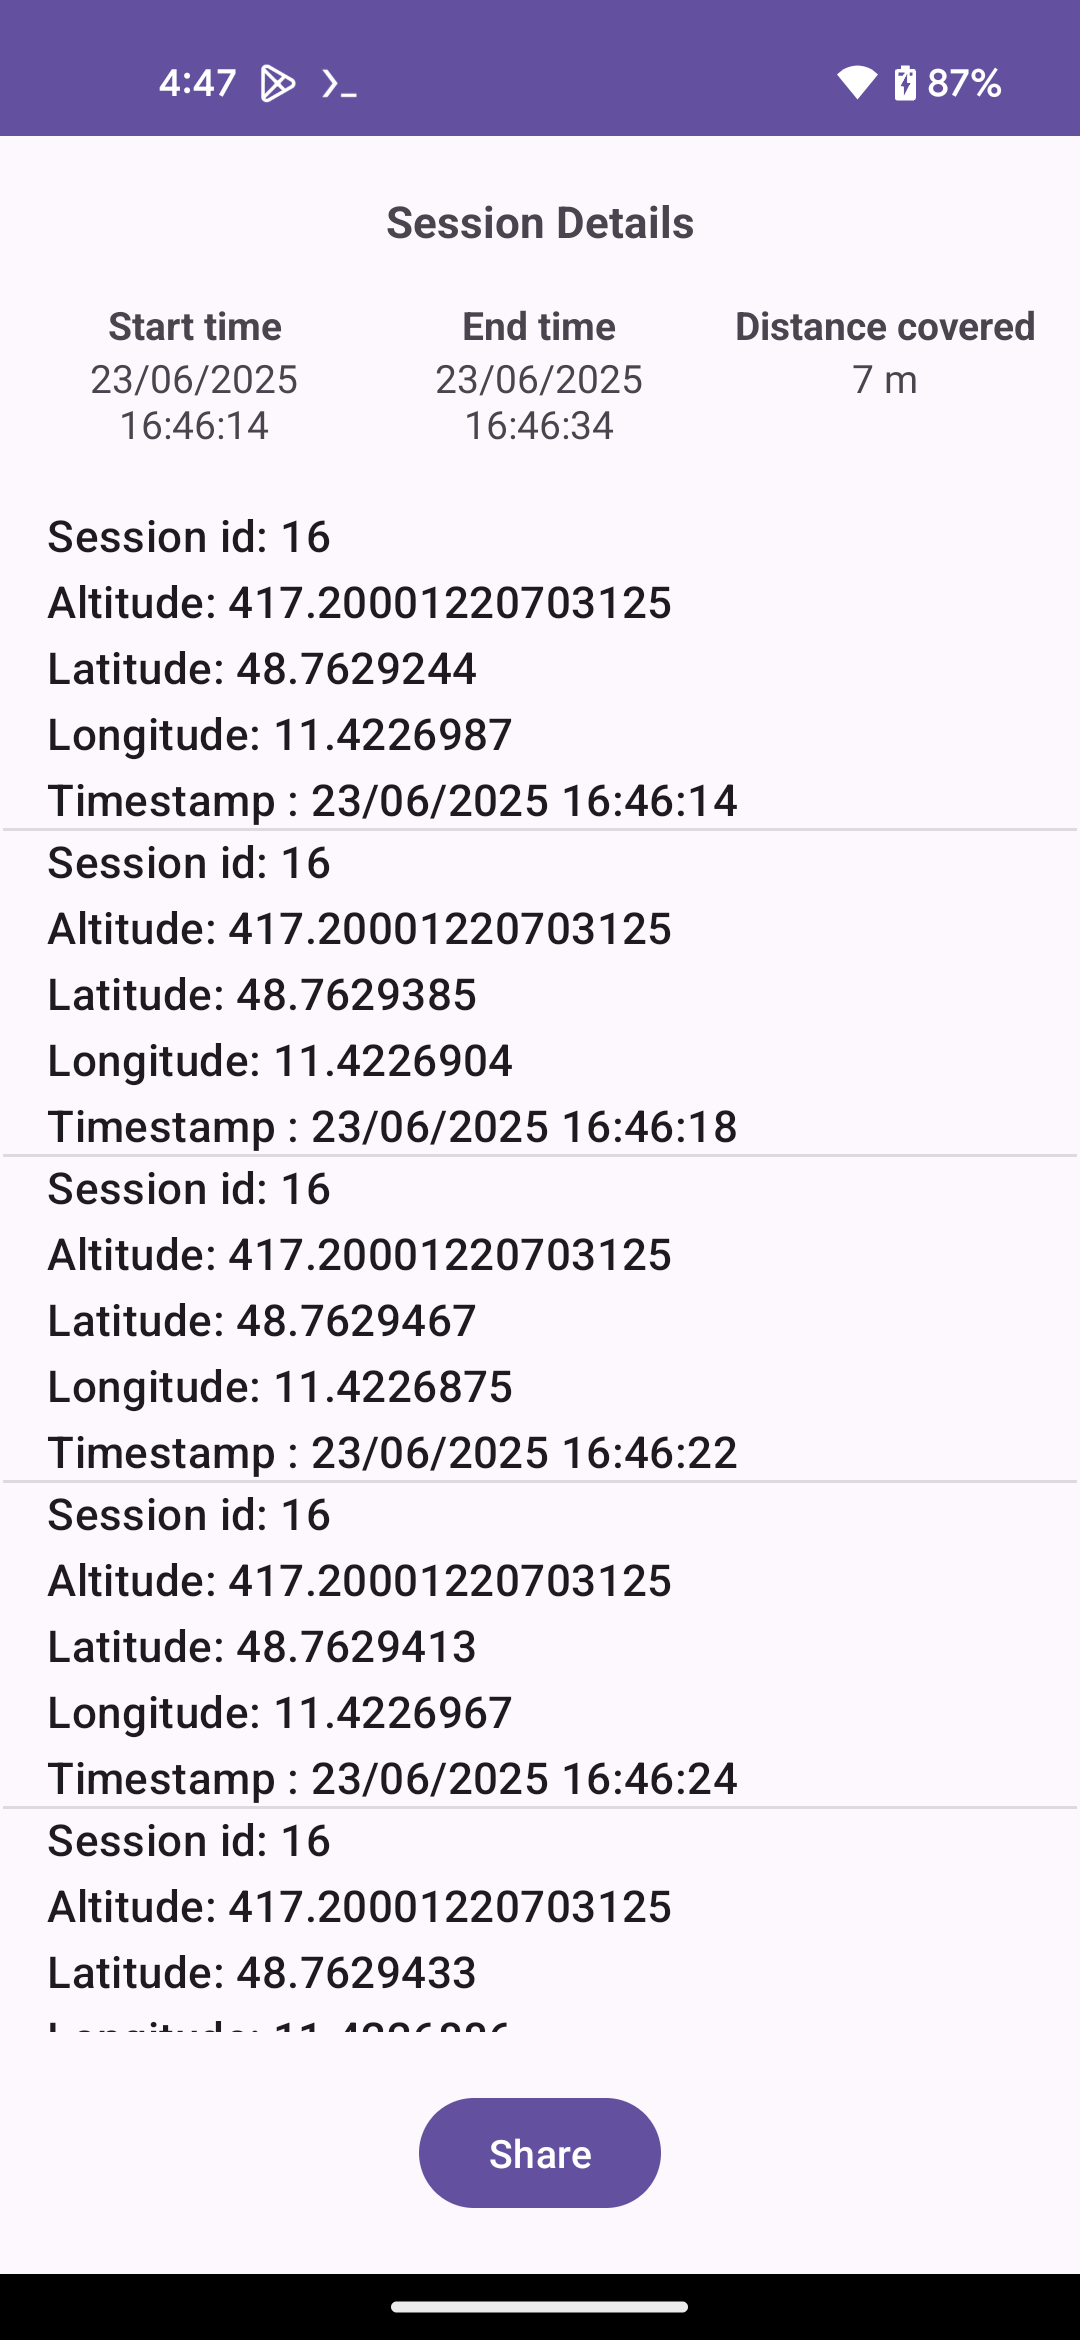
\includegraphics[width=0.23\textwidth]{Project_Screenshots/java4.png}
    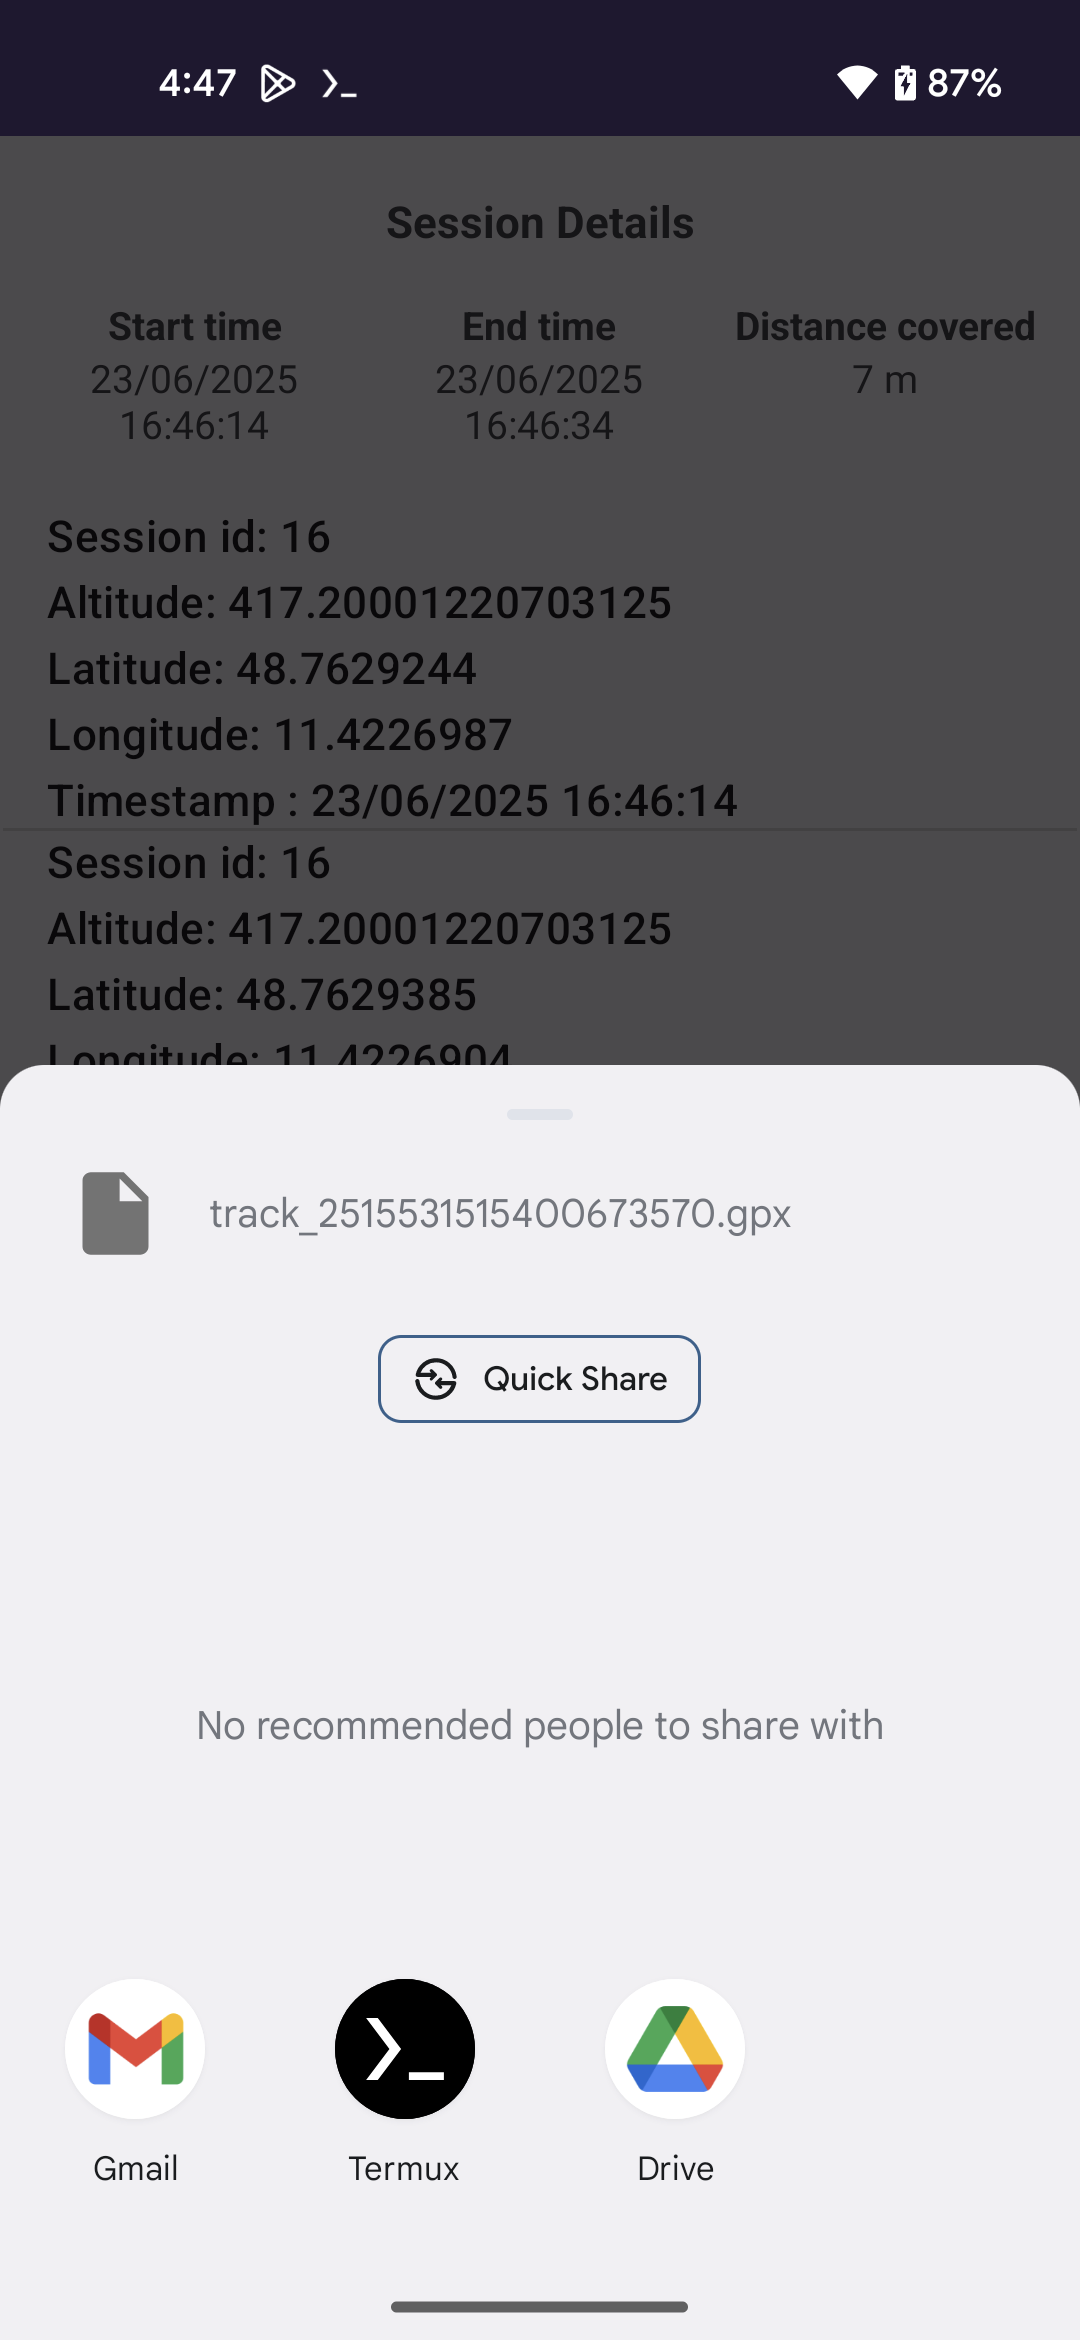
\includegraphics[width=0.23\textwidth]{Project_Screenshots/java5.png}
    \caption{Andriod application GUI by Java}
\end{figure}
\clearpage
\section{GitHub Repository Structure}

\subsection*{TrackINJava}
\begin{verbatim}
TrackINJava/
|
|-- .idea/
|-- app/
|-- gradle/
|
|-- .gitignore
|-- build.gradle.kts
|-- gradle.properties
|-- gradlew
|-- gradlew.bat
\end{verbatim}


\subsection*{backend}
\begin{verbatim}
backend/
|
|-- data/
|-- docs/
|-- src/
|-- test/
|
|-- .gitignore
|-- LICENSE
|-- README.md
|-- main.py
|-- poetry.lock
|-- pyproject.toml
|-- requirements.txt
\end{verbatim}

\subsection*{frontend}
\begin{verbatim}
Flutter Application/
|
|-- android/
|-- ios/
|-- lib/
|-- linux/
|-- macos/
|-- test/
|-- web/
|-- windows/
|
|-- .gitignore
|-- .metadata
|-- .README.md
|-- analysis_options.yaml
|-- main.py
|-- pubspec.lock
|-- pubspec.yaml
|-- trackin_icon_v1.png
\end{verbatim}

\subsection*{Docs}
\begin{verbatim}
Task documents/
|
|-- documents/
\end{verbatim}

\subsection*{serverTesting}
\begin{verbatim}
serverTesting/
|
|-- backend/
|-- main.py
|-- render.yaml
|-- requirement.txt

\end{verbatim}

\clearpage
\section{Conclusion}

Throughout the project, we are successful in developing a cross platform tracking application with a detailed focus on altitude data analysis using GNSS-derived coordinates. Despite the time constraints and complexity of the integration of multiple components like frontend, GUI, backend processing, data synchronization and algorithmic comparison -- we were able to achieve working prototype with functionalities. 

Key accomplishments include the implementation of persistent background tracking, alignment and interpolation of GPX tracks, curve smoothing algorithms, and an extensible framework for visualizing and evaluating geospatial data. All components were structured with modularity in mind to allow for easier future extension.

However, due to limited development time and technical requirements, complexity of flutter, some features remain needing improvement. Advanced elevation correction (e.g., AI-assisted smoothing), multi-user data management, and comprehensive UI polishing are among the areas identified for further improvement.

Future work could focus on:
\begin{itemize}
    \item Enhancing real-time data synchronization between devices or with cloud storage.
    \item Integrating elevation correction using machine learning models or external APIs (e.g., Google Elevation, Mapbox Terrain).
    \item Expanding testing across diverse terrain types and recording conditions.
    \item Allow complete customisation of plots in the backend by providing settings in a JSON file

\end{itemize}

In summary, the current version of the app serves as a solid foundation for further development and experimentation. With additional time and resources, it has strong potential to become a robust tool for elevation-aware route tracking and analysis.

\bigskip

\textbf{Acknowledgements:}  
We would like to thank Prof.\ Dr.\ Robert Gold for his guidance and support throughout the course of this project. Special credit goes to all team members—Baatarbileg Erkhembayar, Syed Aayan Ahmed, Robin Roßnagel, Tom Williams, Himanka Ashan, Susheel Kumar, Prashil Rupapara, Isaac Ye, Pamirbek Almazbekov—for their contributions in development, testing, and documentation.






\end{document}
